% Manuscript for Computers & Operations Research / European Journal of Operational Research
% (both Elsevier: elsarticle class). Build: latexmk -pdf main.tex  (or upload paper/ to Overleaf).
\documentclass[review,12pt,authoryear]{elsarticle}

\usepackage[utf8]{inputenc}
\usepackage[T1]{fontenc}
\usepackage{lmodern}
\usepackage{amsmath,amssymb,amsthm}
\usepackage{booktabs,multirow}
\usepackage{graphicx}
\usepackage{xcolor}
\usepackage{algorithm}
\usepackage{algpseudocode}
\usepackage[colorlinks=true,citecolor=blue!45!black,linkcolor=blue!45!black,urlcolor=blue!45!black]{hyperref}
\usepackage{siunitx}
\sisetup{group-separator={,},output-decimal-marker={.}}

% Pending results are never written as numbers: they stay visible until the closed test runs.
\newcommand{\todo}[1]{\textcolor{red}{[TODO: #1]}}
\newcommand{\pending}[1]{\textcolor{orange}{[pending: #1]}}
\newtheorem{proposition}{Proposition}

\journal{Computers \& Operations Research}

\begin{document}

\begin{frontmatter}

\title{Is learning necessary to reduce the search space? A controlled study of ranking,
restriction and coordinated decomposition for single-source capacitated facility location}

\author[1]{Jean Michael Estevez Alvarez\corref{cor1}}
\ead{estevezcodando@gmail.com}
\cortext[cor1]{Corresponding author.}
\affiliation[1]{organization={\todo{affiliation}}, country={Brazil}}

\begin{abstract}
The single-source capacitated facility location problem (SSCFLP) asks which facilities to
open and which single facility serves each customer, under capacity limits. Even instances
with 30 candidate facilities and 150 customers are not solved to optimality by a modern
open-source MILP solver within a minute, because the linear relaxation leaves a gap of
1.6--4.4\% when fixed costs dominate. Machine learning has been proposed to reduce the search
space of such problems, by pruning variables, ranking them, or choosing which part of a solution
to re-optimize. We ask how much of the reported benefit is due to learning and how much to the
underlying search-space reduction, by pairing every learned component with a learning-free
counterpart of the same function under equal wall-clock budgets.

We study three mechanisms. (i) \emph{Pruning} by a facility ranking is unsafe under capacity
coupling: keeping the best known solution reachable in 80\% of the instances required retaining
about 80\% of the facilities, for a graph neural network (GNN) and for the linear relaxation
alike. (ii) An \emph{adaptive expansion} solves nested restricted problems over the ranked
facilities and stops when reduced costs certify that no excluded facility can improve the
incumbent, which yields a proven optimum without solving the full model. (iii) A
\emph{cluster-oriented large neighborhood search} re-optimizes one group of customers at a time
with the rest fixed and capacities discounted; we prove that every accepted move is globally
feasible and charges each fixed cost once, whereas independently solved clusters violated
capacity in every examined instance. A transposition-style memory identifies subproblems that
have already failed.

In validation pilots, all restriction-based methods had a primal integral two to four times lower
than the solver on the full model, and the hybrid of (ii) and (iii) finished 0.5--0.9\% from the
best known solution against 2.4--2.7\%. Learning, however, was not the source of the gain:
ranking facilities by the linear relaxation was numerically at least as good as the GNN in every
method (differences not significant on 16 instances), and
neither a learned nor a GNN-guided subproblem selector separated from a plain rotation. More
than half of the subproblems selected by the neighborhood search were repetitions of already
failed ones. \todo{one sentence with the closed-test result and its significance}. The
experiments use pinned cores, two clocks, frozen data and pre-registered hypotheses, and we also
report what did not transfer when we reconstructed five recent learning-for-optimization
approaches in an open-source stack.
\end{abstract}


\begin{keyword}
Facility location \sep Single-source capacitated facility location \sep
Large neighborhood search \sep Graph neural networks \sep Matheuristics \sep
Machine learning for combinatorial optimization
\end{keyword}

\end{frontmatter}

\section{Introduction}\label{sec:intro}

Deciding where to open distribution centers and which center serves each demand region is a
recurring strategic decision in logistics. When each region must be served by exactly one
center and centers have limited capacity, the decision is the single-source capacitated
facility location problem (SSCFLP). It is NP-hard, and the single-sourcing requirement makes it
markedly harder than its splittable counterpart: once the open set is fixed, the remaining
assignment is still a generalized assignment problem.

Two lines of work address large SSCFLP instances. Matheuristics restrict the problem and solve
the restriction exactly: kernel search ranks variables by the linear relaxation and solves a
sequence of restricted MILPs \citep{guastaroba2014}, and large neighborhood search (LNS)
repeatedly frees part of the solution and re-optimizes it \citep{kong2021}. More recently,
machine learning has been proposed to accelerate exact and heuristic solvers, either by
learning decisions inside branch-and-bound \citep{gasse2019,gupta2020}, by predicting which
variables to fix or explore \citep{nair2020,han2023}, by learning which neighborhood an LNS
should destroy \citep{song2020,sonnerat2021,huang2023}, or by learning which subproblem a local
search should delegate to an existing solver \citep{li2021delegate}.

Our starting point was the most direct of these ideas for facility location: let a graph neural
network rank candidate facilities and solve the problem restricted to the top-ranked ones. Two
observations changed the direction of the study. First, ranking quality did not translate into
safe pruning. On validation instances, the GNN ranked facilities well (AUC 0.95), yet keeping
the best known solution inside the restricted problem in 80\% of the instances required
retaining about 80\% of the candidates; the LP relaxation alone did almost as well, without
training (Section~\ref{sec:res-pruning}). Capacity forces slack to be kept, and under single
sourcing the slack is spread over many facilities. Second, decomposing the customers into
clusters and solving each cluster independently was fast but wrong: the union of the cluster
solutions violated capacity in every instance we examined and, after repair, was 19--29\% more
expensive than the reference.

The study is organized around four questions. RQ1: does progressive restriction of the
facilities improve the quality available over the budget, against the full solver and classical
controls? RQ2: does replacing only the classical ranking by a learned one improve the result?
RQ3: does adding the coordinated neighborhood search after the restriction improve the final
quality or the anytime behavior? RQ4 (exploratory): do repetition, neighborhood reach and
coordination explain part of the observed limitations? RQ1--RQ3 are answered by a pre-registered
closed test; RQ4 and everything about subproblem selection rest on validation pilots.

These observations redirected the study in two ways. First, we use the ranking to \emph{guide} a
search that never leaves the feasible region, rather than to remove parts of the problem.
Second, since the LP relaxation ranked facilities as safely as the GNN, we ask of every learned
component whether a learning-free counterpart with the same function does as well. We study two
mechanisms, each in a learned and a learning-free variant:
\begin{enumerate}
\item an \textbf{adaptive domain expansion} that solves restricted problems over 20, 40, 60 and
100\% of the ranked facilities and stops early when LP reduced costs certify that no excluded
facility can enter a solution better than the incumbent. The ranking is given by a GNN or by the
LP relaxation; kernel search \citep{guastaroba2014} is the classical baseline; and
\item a \textbf{cluster-oriented LNS (CLNS)} that re-optimizes one subproblem at a time (a
cluster, the boundary between two clusters, the customers of an expensive facility, or the
customers with the largest LP regret) with the rest of the solution fixed and the capacities
reduced by the fixed load. Every accepted move is feasible for the full problem and each fixed
cost is charged once. The subproblem is chosen by rotation, by adaptive operator weights, by a
learned regressor or by disagreement with the GNN, and a memory of failed subproblems measures
and avoids repetitions.
\end{enumerate}

\paragraph{Contributions.}
\begin{itemize}
\item \textbf{A controlled comparison} of learned and learning-free search-space reduction for the
SSCFLP, in which each learned component has a counterpart of the same function under the same
budget. A pre-registered test answers RQ1--RQ3 (Section~\ref{sec:res-test}); exploratory pilots
address RQ4 and subproblem selection (Sections~\ref{sec:res-pilot} and~\ref{sec:res-controls}).
\item \textbf{A characterization of failure modes} under capacity coupling: ranking-based pruning
that cannot be both small and safe, uncoordinated decomposition that produces infeasible unions,
and a neighborhood search in which more than half of the selected subproblems had already been
tried without success (Sections~\ref{sec:res-pruning}, \ref{sec:res-decomp}
and~\ref{sec:res-controls}).
\item \textbf{A reproducible implementation with delimited guarantees}: a coordinated
decomposition whose accepted moves are feasible for the full problem, a reduced-cost stopping
rule that lets a restricted solve prove optimality, and an evaluation protocol with pinned cores,
two clocks, frozen data and registered hypotheses (Sections~\ref{sec:method}
and~\ref{sec:experiments}). The reduced-cost argument and the idea of remembering unproductive
subproblems are classical; we use them, we do not claim them.
\end{itemize}
Appendix~\ref{app:reconstructions} reports, as supplementary material with its own scope, what we
observed when reconstructing five recent learning-for-optimization approaches.

In the pre-registered closed test, run twice on different hardware, restricting the search
space by the LP ranking about halved the primal integral of the solver on the full model, while
the same mechanism driven by the learned ranking had a significantly worse primal integral than
its LP-driven counterpart in both rounds and, on dedicated hardware, was numerically above the full
solver. On real instances with up to
850 customers, only the methods with the coordinated neighborhood search came close to the best
known solution on the two largest.
Section~\ref{sec:related} reviews related work; Section~\ref{sec:problem} states the problem, its
relaxation and the capacity coupling; Section~\ref{sec:method} describes the mechanisms;
Section~\ref{sec:experiments} gives the experimental design; Section~\ref{sec:results} reports
the results; Section~\ref{sec:discussion} discusses them and Section~\ref{sec:conclusion}
concludes.

\section{Related work}\label{sec:related}

\paragraph{Exact methods and matheuristics for the SSCFLP.}
\citet{holmberg1999} proposed an exact algorithm and the 71-instance benchmark with published
optima that we use as an external anchor. \citet{ahuja2004} introduced a very large-scale
neighborhood search based on multi-exchange (cycles and paths of reassignments) that respects
capacity and single sourcing. \citet{guastaroba2014} applied kernel search: variables are ranked
by the LP relaxation and a sequence of restricted MILPs over a growing kernel is solved, which is
the classical counterpart of the learned expansion studied here. \citet{kong2021} proposed an
LNS matheuristic with exact subproblems, reporting optimal solutions for 191 of 272 benchmark
instances and average gaps of 0.04--0.22\% across problem variants.
\todo{check the full texts for numbers before citing them; add recent SSCFLP Lagrangian and
Benders references after a systematic search}.

\paragraph{Learning inside solvers.}
\citet{bengio2021} organize the ways learning and optimization can be combined. Imitation of
strong branching with a graph convolutional network over the variable--constraint graph
\citep{gasse2019} and its CPU-oriented hybrid \citep{gupta2020} are the reference approaches for
learned branching; \citet{chen2025gnnbranching} characterize when message-passing GNNs can
represent strong branching, and \citet{zhou2025subgraph} show that more expressive subgraph GNNs
did not translate into faster solving. Neural diving and neural branching scaled these ideas to
large industrial MIPs \citep{nair2020}. Predict-and-search uses GNN marginals to define a trust
region instead of irreversible fixings \citep{han2023}.

\paragraph{Learned large neighborhood search and delegation.}
LNS policies can be learned by imitation or reinforcement learning \citep{song2020},
from expensive experts \citep{sonnerat2021}, by contrastive learning \citep{huang2023}, with
sampling-enhanced proposals \citep{feng2025spl} or with adaptive neighborhood sizes
\citep{xu2025hypaso}. Learning to delegate selects spatial subproblems of a vehicle routing
problem and hands them to an existing solver, reporting 10--100$\times$ speedups from the
decomposition and 1.5--2$\times$ from the learned selection \citep{li2021delegate}. GLOP
partitions large routing problems before constructing routes \citep{ye2024glop}. Adaptive large
neighborhood search with roulette-wheel operator weights \citep{ropke2006} is the classical
operator-selection baseline. Closest to our setting, \citet{gjergji2026} study an LNS for the
capacitated $p$-median problem with several destruction operators, an exact solver in the repair
step and hyper-heuristics that select among the operators. Our work differs in three respects:
the problem has fixed costs and a free number of facilities, so that neighborhoods must be able
to open and close facilities without double-counting their cost
(Proposition~\ref{prop:feasible}); the search starts from a restricted exact solve with an
optimality certificate rather than from a constructive solution; and every learned component is
compared with a learning-free counterpart of the same function. To our knowledge, learned
subproblem selection has not been studied for capacitated facility location with single
sourcing, where capacity couples the subproblems; the closest classical idea is kernel search
\citep{guastaroba2014}, which we include as a baseline.

\paragraph{Learning for facility location.}
Recent work learns swap policies for $p$-median and facility relocation \citep{guo2023swap},
knowledge-informed swap selection for urban facility location \citep{su2024urban}, Pareto-set
prediction for multi-objective location \citep{liu2022pareto}, and message-passing networks with
approximation guarantees for uniform facility location \citep{qian2026unifl}. Among the works cited here, these address
uncapacitated or accessibility-based variants rather than single-source capacity.

\paragraph{Evaluation of learned optimization methods.}
The primal integral \citep{berthold2013} measures solution quality over time. Instance space
analysis \citep{smithmiles2023} studies where algorithms succeed. We follow both and add timing
controls motivated by an audit of our own implementation (Section~\ref{sec:protocol}).

\section{Problem}\label{sec:problem}

\subsection{Formulation}
Let $I=\{1,\dots,m\}$ be the set of candidate facilities and $J=\{1,\dots,n\}$ the set of
customers. Table~\ref{tab:notation} lists the notation. Opening facility $i$ costs $f_i\ge 0$ and
provides capacity $Q_i>0$; customer $j$ has demand $d_j>0$; serving \emph{all} of $j$'s demand
from $i$ costs $c_{ij}\ge 0$. We stress that $c_{ij}$ is a total cost per pair, not a cost per
unit: in our instances $c_{ij}=\kappa\,\mathrm{dist}_{ij}\,d_j$, and the per-unit cost
$u_{ij}=c_{ij}/d_j$ is used only to compare customers of different sizes. With $y_i=1$ if
facility $i$ opens and $x_{ij}=1$ if $i$ serves $j$, the strict single-source capacitated
facility location problem (SSCFLP) is
\begin{align}
z^\ast=\min\ & \sum_{i\in I} f_i y_i + \sum_{i\in I}\sum_{j\in J} c_{ij} x_{ij} \label{eq:obj}\\
\text{s.t.}\ & \sum_{i\in I} x_{ij} = 1 && j\in J, \label{eq:assign}\\
& \sum_{j\in J} d_j x_{ij} \le Q_i y_i && i\in I, \label{eq:cap}\\
& x_{ij} \le y_i && i\in I,\ j\in J, \label{eq:link}\\
& x_{ij}\in\{0,1\},\quad y_i \in \{0,1\} && i\in I,\ j\in J. \label{eq:int}
\end{align}
The objective \eqref{eq:obj} adds the fixed cost of the open facilities to the cost of the chosen
pairs. Constraints \eqref{eq:assign} assign each customer to exactly one facility; together with
$x_{ij}\in\{0,1\}$ this is the \emph{single-source} requirement, which forbids splitting a demand
among facilities. Constraints \eqref{eq:cap} limit the load of an open facility to its capacity
and force the load of a closed facility to zero. Constraints \eqref{eq:link} are implied by
\eqref{eq:cap} for integer solutions, but they are not implied in the linear relaxation, where
they remove fractional solutions that open a small fraction of a facility and still assign whole
customers to it. Every customer must be served: there is no penalty variable for unmet demand,
which is why we call the problem \emph{strict}.

Because of \eqref{eq:assign} and \eqref{eq:int}, a solution is fully described by an
\emph{assignment} $a:J\to I$, with $x_{ij}=1$ iff $a(j)=i$ and $y_i=1$ iff $i\in a(J)$. Writing
$\ell_i(a)=\sum_{j:\,a(j)=i} d_j$ for the load of facility $i$, the assignment is feasible iff
$\ell_i(a)\le Q_i$ for all $i$, and its cost is
\begin{equation}\label{eq:za}
z(a)=\sum_{i\in a(J)} f_i+\sum_{j\in J} c_{a(j)j}.
\end{equation}
All algorithms in this paper manipulate assignments, and every reported cost is $z(a)$ recomputed
from the original data.

\begin{table}[t]\centering\small
\caption{Notation.}\label{tab:notation}
\begin{tabular}{ll}
\toprule
Symbol & Meaning \\
\midrule
$I$, $J$; $m$, $n$ & candidate facilities and customers; their numbers \\
$f_i$, $Q_i$ & fixed cost and capacity of facility $i$ \\
$d_j$ & demand of customer $j$ \\
$c_{ij}$, $u_{ij}=c_{ij}/d_j$ & total and per-unit cost of serving $j$ from $i$ \\
$y_i$, $x_{ij}$ & opening and assignment variables \\
$a$, $\ell_i(a)$, $z(a)$ & assignment, load of $i$ under $a$, cost \eqref{eq:za} \\
$z^\ast$, $z_{\mathrm{BKS}}$ & optimal and best known cost \\
$L$ & optimal value of the strong LP relaxation \\
$v_j$, $w_i$, $s_{ij}$ & duals of \eqref{eq:assign}, \eqref{eq:cap}, \eqref{eq:link} \\
$r_i$, $\bar c_{ij}$ & reduced costs of $y_i$ and $x_{ij}$ in the strong LP \\
$U$ & cost of the incumbent (upper bound) \\
$K\subseteq I$ & set of facilities kept in a restricted problem \\
$F\subseteq J$ & set of free customers of a subproblem \\
$p_i$ & score of facility $i$ (GNN probability or LP value) \\
$T$, $\alpha$ & time budget; share of $T$ given to the expansion \\
\bottomrule
\end{tabular}
\end{table}

\subsection{The strong linear relaxation and its dual}\label{sec:lp}
Replacing \eqref{eq:int} by $0\le x_{ij}$, $0\le y_i\le 1$ gives the \emph{strong LP}, whose
optimal value we denote $L\le z^\ast$. Associate multipliers $v_j$ (free) with \eqref{eq:assign},
$w_i\ge 0$ with \eqref{eq:cap}, $s_{ij}\ge 0$ with \eqref{eq:link}, and $t_i\ge 0$ with
$y_i\le 1$. The dual is
\begin{align}
L=\max\ & \sum_{j\in J} v_j-\sum_{i\in I} t_i \label{eq:dual}\\
\text{s.t.}\ & v_j - d_j w_i - s_{ij} \le c_{ij} && i\in I,\ j\in J, \label{eq:dualx}\\
& Q_i w_i + \sum_{j\in J} s_{ij} - t_i \le f_i && i\in I, \label{eq:dualy}\\
& w_i,\ s_{ij},\ t_i \ge 0. \nonumber
\end{align}
The slacks of \eqref{eq:dualx} and \eqref{eq:dualy} at an optimal dual solution are the
\emph{reduced costs}
\begin{equation}\label{eq:rc}
\bar c_{ij} = c_{ij} - v_j + d_j w_i + s_{ij}\ \ge 0,
\qquad
r_i = f_i - Q_i w_i - \sum_{j\in J} s_{ij} + t_i\ \ge 0 .
\end{equation}
They have a direct reading. $v_j$ is the marginal cost of serving customer $j$; $w_i$ is the price
of one unit of capacity of facility $i$; $s_{ij}$ is the part of the fixed cost of $i$ that the
relaxation charges to the pair $(i,j)$. Thus $\bar c_{ij}$ is how much more expensive the pair
$(i,j)$ is than what the relaxation is willing to pay for serving $j$, once capacity and the
share of the fixed cost are priced in, and $r_i$ is the part of the fixed cost of $i$ that the
customers' willingness to pay does not cover. By complementary slackness, $\bar c_{ij}=0$ for
every pair used by the LP solution and $r_i=0$ for every facility with $0<y_i<1$.
Two uses of \eqref{eq:rc} recur in the paper: $r_i$ certifies that a pruned facility cannot
improve an incumbent (Proposition~\ref{prop:rc}), and $\bar c_{ij}$ measures how badly the
current assignment of a customer disagrees with the relaxation (the regret of
Section~\ref{sec:clns}).

A remark on a tempting shortcut: the quantity $c_{ij}-v_j$, built from the assignment duals
alone, is \emph{not} a usable regret. Since $v_j$ already embeds the capacity price and the
fixed-cost share of the facility serving $j$ in the LP, $c_{ij}-v_j=\bar c_{ij}-d_jw_i-s_{ij}$ is
non-positive on all LP-used pairs and carries no ranking information; in our first implementation
it was negative for every customer. The full reduced cost $\bar c_{ij}$ is the correct quantity.

\subsection{Why the problem is hard in practice}
The SSCFLP contains the generalized assignment problem (fix $y$) and bin packing (equal costs), so
even deciding whether a set of open facilities admits a feasible assignment is NP-complete. This
has a practical consequence for any method that reduces the set of facilities: a restricted
problem can be infeasible although total capacity exceeds total demand.

On the instance families used here (Section~\ref{sec:data}), SCIP~10 with one thread does not
prove optimality within 60~s for $m=30$ and $n=150$; the certified gap $(U-L_{\mathrm{B\&B}})/U$
after 60~s was 1.8--3.6\%, and the strong LP left $(z_{\mathrm{BKS}}-L)/z_{\mathrm{BKS}}$ of
1.6--4.4\% when fixed costs dominate. For $m=50$, $n=200$ the certified gap reached 15.6\% on one
instance.

\subsection{Capacity coupling}\label{sec:coupling}
Let $J=J_1\cup J_2$ be a partition of the customers and let $a_1$, $a_2$ be optimal assignments
of the two subproblems solved independently, each with the full capacities $Q_i$. The combined
assignment $a=a_1\cup a_2$ can fail in two ways:
\begin{align}
\text{(capacity)}\quad & \ell_i(a)=\ell_i(a_1)+\ell_i(a_2) > Q_i \quad\text{with }\ell_i(a_1),\,\ell_i(a_2)\le Q_i, \label{eq:overload}\\
\text{(fixed cost)}\quad & z(a_1)+z(a_2)-z(a)=\sum_{i\in a_1(J_1)\cap a_2(J_2)} f_i\ \ge 0.
\label{eq:double}
\end{align}
For instance, two groups that each send 60 units to a facility of capacity 100 are feasible
separately and infeasible together \eqref{eq:overload}, and the fixed cost of the shared facility
is counted twice in the sum of the subproblem objectives \eqref{eq:double}, so the subproblems
systematically overestimate the cost of sharing and under-use shared facilities. The
coordinated decomposition of Section~\ref{sec:clns} removes both effects by construction, and
Section~\ref{sec:res-decomp} measures what happens without it.

\section{Method}\label{sec:method}

All mechanisms studied here reduce the search space of \eqref{eq:obj}--\eqref{eq:int} in one of
two ways. \emph{Facility restriction} keeps a subset $K\subseteq I$ and solves the problem with
$y_i=0$ for $i\notin K$ (Sections~\ref{sec:gnn}--\ref{sec:kernel}). \emph{Customer restriction}
keeps the current assignment of all customers outside a subset $F\subseteq J$ and re-optimizes
only $F$ (Sections~\ref{sec:clns}--\ref{sec:memory}). The hybrid (Section~\ref{sec:hybrid})
applies the first and then the second. For each mechanism we give a learned and a learning-free
variant, so that the contribution of learning can be isolated.

\subsection{Facility scores}\label{sec:gnn}
A \emph{score} is a vector $p\in\mathbb{R}^m$; facilities are ranked by decreasing $p_i$.

\paragraph{LP score (no learning).} With $(y^{\mathrm{LP}},r)$ the opening values and reduced
costs of the strong LP (Section~\ref{sec:lp}),
\begin{equation}\label{eq:lpscore}
p^{\mathrm{LP}}_i = y^{\mathrm{LP}}_i - \epsilon\,\frac{r_i}{\max_{k\in I}|r_k|},\qquad
\epsilon=10^{-3},
\end{equation}
so that facilities are ordered by their LP opening value and ties among facilities closed in the
LP ($y^{\mathrm{LP}}_i=0$) are broken by increasing reduced cost, i.e., by how little the LP bound
would deteriorate if they were forced open.

\paragraph{Classical score (no learning, no LP).} The service ratio of the greedy \emph{add}
heuristic: let $j_1,j_2,\dots$ be the customers sorted by increasing $u_{ij}$ and $q$ the largest
index with $\sum_{k\le q} d_{j_k}\le Q_i$; then
\begin{equation}
p^{\mathrm{cl}}_i=-\frac{f_i+\sum_{k\le q}c_{ij_k}}{\sum_{k\le q}d_{j_k}},
\end{equation}
the negative of
the average cost per unit of demand when $i$ serves its cheapest customers up to capacity.

\paragraph{GNN score (learned).} Each instance is a bipartite graph $G=(I\cup J,E)$, where $E$
contains the pair $(i,j)$ if $i$ is among the $k=10$ cheapest facilities of $j$ or $j$ is among
the $k=10$ cheapest customers of $i$ (by $u_{ij}$). Node and edge features are normalized by
statistics of the instance itself, so that one model applies across sizes: for facilities,
capacity and fixed cost relative to the instance means, the classical score, local demand
density and a profile-based competition count; for customers, demand, cheapest unit cost and
regret; for edges, the unit cost $u_{ij}$ and its rank from both endpoints.
Initial embeddings are $h^{0}_i=\phi_I(\mathbf{x}_i)$, $h^{0}_j=\phi_J(\mathbf{x}_j)$,
$e_{ij}=\phi_E(\mathbf{x}_{ij})$ in $\mathbb{R}^{64}$. Each of $R=3$ rounds updates customers
from facilities and then facilities from customers:
{\small
\begin{align}
\mu^{t}_{ij} &= \psi^{t}_{IJ}\bigl([h^{t}_i,e_{ij}]\bigr), &
m^{t}_{j} &= \Bigl[\tfrac{1}{|N(j)|}\textstyle\sum_{i\in N(j)}\mu^{t}_{ij},\
\tfrac{1}{\Delta_J}\sum_{i\in N(j)}\mu^{t}_{ij}\Bigr], \nonumber\\
&& h^{t+1}_j &= \mathrm{LN}\bigl(h^{t}_j+\gamma^{t}_{J}([h^{t}_j,m^{t}_j])\bigr), \label{eq:mpj}\\
\nu^{t}_{ji} &= \psi^{t}_{JI}\bigl([h^{t+1}_j,e_{ij}]\bigr), &
m^{t}_{i} &= \Bigl[\tfrac{1}{|N(i)|}\textstyle\sum_{j\in N(i)}\nu^{t}_{ji},\
\tfrac{1}{\Delta_I}\sum_{j\in N(i)}\nu^{t}_{ji}\Bigr], \nonumber\\
&& h^{t+1}_i &= \mathrm{LN}\bigl(h^{t}_i+\gamma^{t}_{I}([h^{t}_i,m^{t}_i])\bigr), \label{eq:mpi}
\end{align}}
where $N(\cdot)$ is the neighborhood in $G$, $\Delta_J$ and $\Delta_I$ are the maximum degrees
(so the second aggregate is a sum normalized to $[0,1]$, which keeps degree information that the
mean discards), $\psi$, $\gamma$ and $\phi$ are two-layer perceptrons, $[\cdot,\cdot]$ is
concatenation and $\mathrm{LN}$ is layer normalization. The output is one logit per facility,
$p^{\mathrm{GNN}}_i=\eta(h^{R}_i)$. Conditioning messages on $e_{ij}$ matters because the
relevant information (how expensive $i$ is for $j$ relative to $j$'s alternatives) lives on the
edges.

The target is a \emph{soft} label that tolerates alternative optima. Let $\mathcal{P}$ be the
pool of solutions found for a training instance by SCIP (60~s) and LNS (30~s), and
$\mathcal{P}_{\tau}=\{a\in\mathcal{P}: z(a)\le(1+\tau)\min_{a'\in\mathcal{P}}z(a')\}$ with
$\tau=1\%$. The label of facility $i$ is the frequency with which it is open in near-best
solutions,
\begin{equation}\label{eq:label}
q_i=\frac{1}{|\mathcal{P}_{\tau}|}\sum_{a\in\mathcal{P}_{\tau}}\mathbf{1}[\,i\in a(J)\,]\in[0,1],
\end{equation}
and the loss is the class-balanced binary cross-entropy
\begin{equation}\label{eq:loss}
\mathcal{L}=-\frac{1}{m}\sum_{i\in I}\omega_i\Bigl[q_i\log\sigma(p_i)+(1-q_i)\log\bigl(1-\sigma(p_i)\bigr)\Bigr],
\qquad
\omega_i=\begin{cases}\dfrac{1}{2\pi} & q_i>\tfrac12,\\[2mm] \dfrac{1}{2(1-\pi)} & \text{otherwise,}\end{cases}
\end{equation}
with $\sigma$ the logistic function and $\pi=\min\{0.98,\max\{0.02,\frac1m\sum_i q_i\}\}$ the
mean label of the instance; the weights $\omega_i$ give open and closed facilities the same total
weight, since typically fewer than half of the facilities are open. We train three seeds with
early stopping on validation instances.

\subsection{Restricted problems and feasibility repair}\label{sec:repair}
For $K\subseteq I$, the restricted problem $\mathrm{P}(K)$ is \eqref{eq:obj}--\eqref{eq:int} with
$y_i=0$ for $i\notin K$; its optimal value satisfies $z^\ast(K)\ge z^\ast$, with equality iff
some optimal solution opens only facilities of $K$. Given a ranking and a target fraction
$\rho\in(0,1]$, we take the $\lceil\rho m\rceil$ best facilities and \emph{repair} the set in two
steps, adding facilities in ranking order:
\begin{enumerate}
\item \emph{Packing.} Add facilities until the first-fit-decreasing heuristic (customers by
decreasing demand, each placed in the first kept facility with enough residual capacity) packs
all demands. This is a sufficient condition for $\mathrm{P}(K)$ to be feasible; the necessary
condition $\sum_{i\in K}Q_i\ge\sum_j d_j$ is not sufficient under single sourcing.
\item \emph{Coverage.} For every customer with none of its five cheapest facilities in $K$, add
the best-ranked of those five.
\end{enumerate}
We denote the result $\mathrm{rep}(\rho)$. On our instances the repair alone keeps at least 41\%
of the facilities, so a nominal $\rho=0.2$ does not yield a problem five times smaller; this
lower bound on the kept fraction is a property of capacitated instances, not of the ranking.

\subsection{Adaptive expansion with a reduced-cost certificate}\label{sec:expansion}
Let $\rho_1<\rho_2<\rho_3<\rho_4$ be $0.2,0.4,0.6,1$ and $K_s=\mathrm{rep}(\rho_s)\cup a^{s-1}(J)$,
where $a^{s-1}$ is the incumbent after stage $s-1$ (so the incumbent is always feasible for the
next stage) and $K_4=I$. Stage $s$ solves $\mathrm{P}(K_s)$ with SCIP, warm-started with
$a^{s-1}$, for a quarter of the remaining budget (the last stage receives all of it).

\begin{proposition}[Reduced-cost exclusion]\label{prop:rc}
Let $L$ be the optimal value of the strong LP and $r_i\ge0$ the reduced cost \eqref{eq:rc} of
$y_i$ at an optimal dual solution. Every feasible solution of
\eqref{eq:obj}--\eqref{eq:int} with $y_i=1$ has cost at least $L+r_i$. Consequently, if
$L+r_i\ge U$ for an incumbent of cost $U$, no solution that opens $i$ is better than the
incumbent.
\end{proposition}
\begin{proof}
Let $(v,w,s,t)$ be an optimal dual solution and $(x,y)$ any LP-feasible point. Substituting
$f_k=r_k+Q_kw_k+\sum_j s_{kj}-t_k$ and $c_{kj}=\bar c_{kj}+v_j-d_jw_k-s_{kj}$ from \eqref{eq:rc}
into the objective and regrouping by multiplier,
\begin{align*}
\sum_{k} f_k y_k+\sum_{k,j} c_{kj}x_{kj}
={}& \sum_k r_ky_k+\sum_{k,j}\bar c_{kj}x_{kj}+\sum_j v_j\underbrace{\sum_k x_{kj}}_{=1}
+\sum_k w_k\underbrace{\Bigl(Q_ky_k-\sum_j d_jx_{kj}\Bigr)}_{\ge0}\\
&+\sum_{k,j}s_{kj}\underbrace{(y_k-x_{kj})}_{\ge0}-\sum_k t_k\underbrace{y_k}_{\le1}\\
\ge{}& \Bigl(\sum_j v_j-\sum_k t_k\Bigr)+\sum_k r_ky_k+\sum_{k,j}\bar c_{kj}x_{kj}
\ \ge\ L+r_iy_i ,
\end{align*}
where the last step uses strong duality \eqref{eq:dual} and $r_k,\bar c_{kj}\ge0$. Every integer
solution is LP-feasible, so $y_i=1$ gives cost at least $L+r_i$.
\end{proof}

\noindent\emph{Certificate.} If stage $s$ solves $\mathrm{P}(K_s)$ to optimality with value $U$
and
\begin{equation}\label{eq:cert}
L+r_i\ \ge\ U\qquad\text{for all } i\in I\setminus K_s,
\end{equation}
then $U=z^\ast$: a better solution would have to open some pruned facility, which
Proposition~\ref{prop:rc} excludes. The expansion then stops with a \emph{proven} global optimum
although only a fraction of the facilities entered the solver. \emph{Guided expansion.} When
\eqref{eq:cert} fails, the set $\{i\notin K_{s}: L+r_i<U\}$ of facilities that the certificate
cannot exclude is added to the next stage, provided the stage does not exceed $1.5\,\rho_{s+1}m$
facilities. The LP is solved once (HiGHS) and its duals are reused by every later component.

With $p=p^{\mathrm{GNN}}$ this is the learned expansion; with $p=p^{\mathrm{LP}}$
\eqref{eq:lpscore} nothing is learned and the method becomes a variant of kernel search with
nested kernels, which is the natural control for the value of the GNN.

\subsection{Kernel search}\label{sec:kernel}
As the classical counterpart we implement kernel search \citep{guastaroba2014} over facilities.
The initial kernel is $\Lambda_0=\mathrm{rep}$ of $\{i: y^{\mathrm{LP}}_i>0\}$. The remaining
facilities, sorted by increasing reduced cost $r_i$, are cut into buckets
$B_1,\dots,B_q$ of size $|\Lambda_0|$. The method solves $\mathrm{P}(\Lambda_0)$ and then, for
$b=1,\dots,q$, the problem $\mathrm{P}(\Lambda_{b-1}\cup B_b)$ warm-started with the incumbent
$a$, and updates
\begin{equation}
\Lambda_b=\Lambda_{b-1}\cup\bigl(B_b\cap a(J)\bigr),
\end{equation}
i.e., a bucket facility joins the kernel only if the new incumbent uses it. The kernel problem
receives 25\% of the remaining time and each bucket an equal share of what is left. Unlike the
original, we do not add the constraint $\sum_{i\in B_b}y_i\ge1$ nor an objective cutoff; the
warm start plays the role of the cutoff. The difference from the adaptive expansion is
structural: kernel search visits \emph{disjoint} buckets around a small kernel and never solves
the full problem, whereas the expansion solves \emph{nested} sets and ends with $K=I$.

\subsection{Cluster-oriented large neighborhood search}\label{sec:clns}
\paragraph{Clusters.} Customers are clustered once by $k$-means on the log-scaled unit-cost
profile $\xi_j=\bigl(\log(1+u_{ij}/\tilde u)\bigr)_{i\in I}\in\mathbb{R}^m$, with $\tilde u$ the
median of all $u_{ij}$ and $k=\mathrm{round}(n/15)$:
\begin{equation}
\min_{G_1,\dots,G_k}\ \sum_{g=1}^{k}\sum_{j\in G_g}\lVert \xi_j-\mu_g\rVert_2^2,\qquad
\mu_g=\frac{1}{|G_g|}\sum_{j\in G_g}\xi_j .
\end{equation}
Two customers are close when they see the facilities at similar prices, which is the relevant
notion of proximity for exchanging them between facilities and does not require coordinates
(the Holmberg instances have none). The distance between clusters $g$ and $h$ is the
$\ell_1$ distance between their mean unit-cost profiles.

\paragraph{Subproblem.} Given a feasible assignment $a$ and a set $F\subseteq J$ of \emph{free}
customers, let $\bar F=J\setminus F$,
\begin{equation}\label{eq:resid}
\ell^{\bar F}_i=\sum_{j\in\bar F:\ a(j)=i}d_j,\qquad
\tilde Q_i=Q_i-\ell^{\bar F}_i,\qquad
I^{\mathrm{paid}}=a(\bar F),
\end{equation}
be the load of the fixed customers, the residual capacity, and the facilities whose fixed cost is
already paid by a fixed customer. Each free customer $j$ may use the set $C_j$ of its ten cheapest
facilities plus its current one $a(j)$. The subproblem $\mathrm{S}(a,F)$ is
\begin{align}
\min\ & \sum_{i\notin I^{\mathrm{paid}}} f_i y_i+\sum_{j\in F}\sum_{i\in C_j} c_{ij}x_{ij}
\label{eq:subobj}\\
\text{s.t.}\ & \sum_{i\in C_j}x_{ij}=1 && j\in F, \nonumber\\
& \sum_{j\in F:\ i\in C_j} d_jx_{ij}\le \tilde Q_i\,y_i && i\notin I^{\mathrm{paid}}, \nonumber\\
& \sum_{j\in F:\ i\in C_j} d_jx_{ij}\le \tilde Q_i && i\in I^{\mathrm{paid}}, \nonumber\\
& x_{ij}\le y_i && i\notin I^{\mathrm{paid}},\ j\in F,\ i\in C_j, \nonumber\\
& x_{ij},y_i\in\{0,1\}. \nonumber
\end{align}
SCIP solves it starting from $a|_F$ (always feasible, since $a(j)\in C_j$) with a short time limit
$\theta$: $\theta=0.5$~s, multiplied by $1+0.5\min\{\phi,4\}$ after $\phi$ consecutive failures.
The move is accepted only if it strictly improves the full objective \eqref{eq:za}.

\begin{proposition}[Coordination]\label{prop:feasible}
Let $a$ be feasible and $a'$ be obtained from $a$ by replacing $a|_F$ with a feasible solution of
$\mathrm{S}(a,F)$ of value $\zeta'$. Then $a'$ is feasible for
\eqref{eq:obj}--\eqref{eq:int} and
\begin{equation}\label{eq:delta}
z(a')=\zeta'+\underbrace{\sum_{i\in I^{\mathrm{paid}}}f_i+\sum_{j\in\bar F}c_{a(j)j}}_{\text{constant in }F},
\qquad\text{so}\qquad z(a)-z(a')=\zeta-\zeta',
\end{equation}
where $\zeta$ is the value of $a|_F$ in $\mathrm{S}(a,F)$.
\end{proposition}
\begin{proof}
Single sourcing holds because each free customer receives exactly one facility and fixed
customers keep theirs. For capacity, $\ell_i(a')=\ell^{\bar F}_i+\sum_{j\in F}d_jx_{ij}\le
\ell^{\bar F}_i+\tilde Q_i=Q_i$. For the cost, a facility in $I^{\mathrm{paid}}$ is open in both
$a$ and $a'$ and contributes $f_i$ once to the constant; a facility outside
$I^{\mathrm{paid}}$ is open in $a'$ iff some free customer uses it, i.e., iff $y_i=1$ in an
optimal completion of the subproblem, so its fixed cost is counted exactly once, in $\zeta'$.
\end{proof}
\noindent Proposition~\ref{prop:feasible} is what separates the CLNS from the naive
decomposition of Section~\ref{sec:coupling}: residual capacities rule out the overload
\eqref{eq:overload} and the set $I^{\mathrm{paid}}$ rules out the double counting
\eqref{eq:double}. It also shows that the improvement of the full objective equals the
improvement of the subproblem, so no global evaluation is needed to decide acceptance.

\paragraph{Candidate subproblems.} At each iteration a set $\mathcal{F}(a)$ of candidate free
sets is built from the incumbent:
\begin{itemize}
\item \emph{interior}: $F=G_g$ for each cluster $g$;
\item \emph{boundary}: $F=G_g\cup G_h$ for each cluster $g$ and its nearest cluster $h$, which
allows transfers between clusters;
\item \emph{release}: for the six open facilities with the largest fixed cost per unit of load
$f_i/\ell_i(a)$, the customers of $i$ and of the two open facilities with the closest unit-cost
profiles (subsampled to the customers of $i$ plus 30 others when the set exceeds 45
customers). This is the move that can \emph{close} a facility whose customers are spread over
several clusters, which interior and boundary moves cannot;
\item \emph{regret}: for the four customers with the largest LP regret
\begin{equation}\label{eq:regret}
\varrho_j(a)=\bar c_{a(j)j}-\min_{i\in I}\bar c_{ij}\ \ge 0,
\end{equation}
the 15 customers closest to $j$ in unit-cost profile. $\varrho_j$ is zero when $j$ is assigned as
in the LP and grows with the price the relaxation attaches to the current choice;
\item \emph{opening} (only when a GNN score is available): for the four closed facilities with the
highest $p_i$, their 15 cheapest customers.
\end{itemize}

\subsection{Choosing the subproblem}\label{sec:selectors}
A \emph{selector} maps $\mathcal{F}(a)$ and the search history to one candidate.
\emph{Rotation} cycles through the types and draws a candidate uniformly within the type.
\emph{ALNS} \citep{ropke2006} draws a type $\tau$ with probability
$\pi_\tau=\omega_\tau/\sum_{\tau'}\omega_{\tau'}$ and updates the weights every ten iterations,
\begin{equation}
\omega_\tau\leftarrow\max\bigl\{0.05,\ (1-\lambda)\,\omega_\tau+\lambda\,\bar s_\tau\bigr\},
\qquad \lambda=0.2,
\end{equation}
where $\bar s_\tau$ is the fraction of improving moves of type $\tau$ in the segment.
\emph{Dual} picks the candidate with the largest mean regret
$\frac{1}{|F|}\sum_{j\in F}\varrho_j(a)$, halved for each previous failure of that candidate.
\emph{Learned} follows learning-to-delegate \citep{li2021delegate}: a gradient-boosted regressor
$\hat g$ predicts the improvement per second of a candidate from 16 features of $(a,F)$ and the
selector takes $\arg\max_{F\in\mathcal{F}(a)}\hat g(a,F)$ (Section~\ref{sec:training}).
\emph{GNN-guided} needs no additional training and picks the candidate whose current
configuration most disagrees with the facility scores. With
$\hat p_i=\sigma(p^{\mathrm{GNN}}_i)$,
\begin{equation}\label{eq:delta-gnn}
\delta(F)=\frac{\sum_{i\in O(F)}(1-\hat p_i)+\sum_{i\in C(F)}\hat p_i}{|O(F)|+|C(F)|},
\qquad
F^\ast=\arg\max_{F\in\mathcal{F}(a)}\ \delta(F)\,2^{-\varphi(F)},
\end{equation}
where $O(F)=a(F)$ are the open facilities serving $F$, $C(F)$ are the closed facilities among the
three cheapest of each customer in $F$, and $\varphi(F)$ counts the failures of $F$ since the
last improvement. The first sum is large when $F$ is served by facilities the model considers
unlikely; the second when likely facilities nearby are closed.

\subsection{Subproblem memory}\label{sec:memory}
An LNS that accepts only improvements can select the same subproblem repeatedly from an
unchanged neighborhood. By \eqref{eq:resid}--\eqref{eq:subobj}, $\mathrm{S}(a,F)$ depends on $a$
only through $a|_F$ (which fixes the sets $C_j$ and the starting solution) and through the fixed
loads $(\ell^{\bar F}_i)_{i\in I}$ (which fix $\tilde Q$ and $I^{\mathrm{paid}}=\{i:\ell^{\bar F}_i>0\}$).
We therefore define the key
\begin{equation}\label{eq:key}
\kappa(a,F)=H\bigl(F,\ a|_F,\ (\ell^{\bar F}_i)_{i\in I}\bigr),
\end{equation}
with $H$ a 96-bit hash, and keep a table $M:\kappa\mapsto\theta_{\max}$ of the largest time limit
with which the subproblem failed to improve.

\begin{proposition}\label{prop:key}
If $\bigl(F,a|_F,\ell^{\bar F}\bigr)=\bigl(F,b|_F,\ell'^{\bar F}\bigr)$ for two feasible assignments
$a$ and $b$, then $\mathrm{S}(a,F)$ and $\mathrm{S}(b,F)$ are the same mixed-integer program with
the same starting solution.
\end{proposition}
\noindent The proof is by inspection of \eqref{eq:resid}--\eqref{eq:subobj}. Note that the key is
\emph{coarser} than the full assignment: two assignments that differ in how fixed customers are
distributed, but produce the same fixed loads, share the key. With memory enabled, candidates
with $M[\kappa(a,F)]\ge\theta$ are removed from $\mathcal{F}(a)$ before selection (unless all are
removed); a failure with a larger limit $\theta$ is still allowed, since the solver may improve
with more time. This is the transposition table of game-tree search applied to neighborhoods:
it does not change which solutions are reachable, only avoids paying twice for the same negative
answer. With memory disabled we still compute the key of the selected candidate to
\emph{measure} the repetition rate, reported in Section~\ref{sec:res-controls}.

\subsection{The hybrid}\label{sec:hybrid}
Algorithm~\ref{alg:hybrid} runs the adaptive expansion for a share $\alpha$ of the budget
($\alpha=0.5$, fixed before the experiments) and the CLNS for the rest, from the expansion's
solution, reusing the LP duals and, for the GNN-guided selector, the facility scores.

\begin{algorithm}[t]
\caption{Hybrid: adaptive expansion followed by CLNS}\label{alg:hybrid}
\begin{algorithmic}[1]
\Require instance, budget $T$, share $\alpha$, score type (GNN or LP), selector, memory flag
\State $p \gets$ facility scores; solve strong LP $\to (L, r, \bar c)$
\State $a \gets$ \textsc{AdaptiveExpansion}$(p, L, r)$ with budget $\alpha T$
\Comment{Section~\ref{sec:expansion}}
\State clusters $\gets$ $k$-means on unit-cost profiles; $M\gets\emptyset$; $\phi\gets0$
\While{time remains}
  \State $\theta\gets0.5\,(1+0.5\min\{\phi,4\})$
  \State $\mathcal{F} \gets$ candidate subproblems of $a$ (five types)
  \If{memory} $\mathcal{F}\gets\{F\in\mathcal{F}: M[\kappa(a,F)]<\theta\}$ (if non-empty) \EndIf
  \State $F \gets$ \textsc{Select}$(\mathcal{F})$ \Comment{Section~\ref{sec:selectors}}
  \State $a' \gets$ solve $\mathrm{S}(a,F)$ for at most $\theta$ seconds
  \If{$z(a') < z(a)$} $a \gets a'$; $\phi\gets0$
  \Else\ $M[\kappa(a,F)]\gets\max\{M[\kappa(a,F)],\theta\}$; $\phi\gets\phi+1$ \EndIf
\EndWhile
\State \Return $a$ (validated against the original data)
\end{algorithmic}
\end{algorithm}

\subsection{Training the learned selector}\label{sec:training}
Labels are collected \emph{off-policy}: at states visited by a reasonable search on 60 training
instances, eight candidates drawn uniformly from $\mathcal{F}(a)$ are solved from the \emph{same}
state and, for each, the features, the improvement $\Delta_F=z(a)-z(a'_F)\ge0$ and the time
$\tau_F$ are recorded; the search then continues from the best of the eight. Solving several
candidates from the same state gives counterfactual labels that an on-policy trace (one candidate
per state) cannot provide. The regression target is the normalized improvement per second,
\begin{equation}
g(a,F)=\frac{\Delta_F/\tilde c}{\max\{\tau_F,\,0.05\}},
\end{equation}
with $\tilde c$ the median pair cost of the instance, so that targets are comparable across
instances. The 16 features are: share of customers and of demand in $F$; mean cost of $F$; mean
and maximum regret \eqref{eq:regret}; number of facilities involved; capacity slack and fixed
cost per unit of load of those facilities; attempts, cumulative gain and age of the candidate;
the capacity ratio of the instance; and the candidate type. This yielded 23{,}840 training and
6{,}256 validation labels (11.7\% with $\Delta_F>0$), split by instance. The regressor reached
AUC 0.76 for predicting $\Delta_F>0$ on held-out instances; the most important features were
capacity slack and fixed cost per unit of load.

\section{Experimental design}\label{sec:experiments}

\subsection{Instances}\label{sec:data}
\paragraph{Synthetic families.} We adapt the generator of \citet{cornuejols1991}, also used for
the \texttt{facilities} family of \citet{gasse2019}, to single sourcing:
\begin{itemize}
\item demand $d_j\sim U(5,35)$;
\item raw capacities $U(10,160)$, rescaled to a total-capacity-to-demand ratio
$r\in\{1.5, 3.0\}$;
\item fixed cost $f_i = (U(0,90) + U(100,110)\sqrt{Q_i})$;
\item service cost $c_{ij} = 10\, \mathrm{dist}_{ij}\, d_j$.
\end{itemize}
Customer locations follow three spatial families: uniform, clustered (Gaussian mixture) and
corridor (points along a few segments). Instances infeasible under single sourcing are rejected
by a first-fit-decreasing test followed, if needed, by a feasibility MILP. Splits are disjoint in
generator seeds; the corridor family never appears in training or validation.

\paragraph{External and real instances.} The 71 instances of \citet{holmberg1999}, with
published optima, use non-Euclidean costs and 10--30 facilities by 50--200 customers. The case
study uses delivered orders from the Olist public dataset aggregated by three-digit postal-code
prefix (up to 850 regions and 150 candidate facilities), with freight from the minimum road
freight tariff of the Brazilian regulator (ANTT); capacities and fixed costs are declared
modeling assumptions.

\begin{table}[t]\centering\small
\caption{Data sets. All files are frozen with SHA-256 hashes before any run.}\label{tab:data}
\resizebox{\linewidth}{!}{%
\begin{tabular}{llrll}
\toprule
Set & Size ($|I|\times|J|$) & Instances & Reference & Use \\
\midrule
Train & $30\times150$ & 160 & SCIP 60 s + LNS 30 s pool & GNN and selector training \\
Validation & $30\times150$ & 32 & same & parameter choices \\
Test & $30\times150$ & 32 & same & closed test \\
Corridor & $30\times150$ & 16 & same & unseen spatial family \\
Scale & $50\times200$ & 16 & SCIP 120 s + LNS 60 s & larger size \\
Holmberg & $10$--$30\times50$--$200$ & 71 & published optimum & external anchor \\
Olist & $30\times150$ to $150\times850$ & 4 & SCIP 300 s + LNS 120 s & real data \\
\bottomrule
\end{tabular}}
\end{table}

\subsection{Methods compared}
\begin{itemize}
\item \textbf{SCIP} 10.0 on the full model, one thread, default settings.
\item \textbf{Warm SCIP}: the LNS below for 10\% of the budget, then SCIP from its solution.
\item \textbf{LNS}: a matheuristic that frees customers with similar cost profiles or the
customers of one or two facilities and re-optimizes them with SCIP, with adaptive neighborhood
size.
\item \textbf{Adaptive expansion} alone (Section~\ref{sec:expansion}) over the full budget, with
the GNN score and, as a learning-free control, with the LP score \eqref{eq:lpscore}.
\item \textbf{Kernel search} \citep{guastaroba2014} over facilities (Section~\ref{sec:kernel}),
the classical counterpart of the expansion, with the same budget and solver.
\item \textbf{CLNS} from the LP-rounded start with each selector (rotation, ALNS, learned, GNN).
\item \textbf{Hybrid} (Algorithm~\ref{alg:hybrid}) with the GNN-guided, rotation and learned
selectors; \textbf{LP hybrid}, the same algorithm with the LP score in place of the GNN and the
rotation selector, in which no component is learned.
\item \textbf{Memory} variants (suffix \emph{+mem}) of CLNS and of both hybrids, with the
subproblem memory of Section~\ref{sec:memory}.
\item \textbf{Naive decomposition}: clusters solved independently with full capacities, then
greedily repaired.
\end{itemize}

\subsection{Protocol}\label{sec:protocol}
An audit of an earlier version of our harness found that solver set-up time was counted twice in
incumbent trajectories, that the primal integral did not use the cumulative best incumbent across
stages, and that there was no global deadline. The corrected protocol, frozen before the runs
reported here, is:
\begin{itemize}
\item \textbf{Equal wall-clock budget} per method (60~s for $30\times150$ and corridor, 120~s for
$50\times200$, 30~s for Holmberg), including feature computation, inference, LP, repair, model
building, solving and validation, under one monotonic clock.
\item \textbf{Isolation}: each run on a dedicated physical core (CPU affinity), with one core left
for the operating system, all numerical libraries limited to one thread, and imports and models
warmed up outside the timed region.
\item \textbf{Two clocks}: wall-clock and process CPU time. The ratio CPU/wall flags runs that
waited for the CPU; runs below 0.9 are marked as suspected contention.
\item \textbf{Frozen data}: instances and models are hashed in a versioned lock file; every run
verifies the lock and records the aggregate hash in its manifest.
\item \textbf{Seeds}: three solver seeds for stochastic methods, one for deterministic ones; seeds
are averaged within an instance before any statistics across instances. Three GNN checkpoints
were trained, but all optimization runs use the checkpoint of training seed 0; conclusions about
the learned ranking are limited to that checkpoint. Three GNN checkpoints
were trained, but all optimization runs use the checkpoint of training seed 0; conclusions about
the learned ranking are limited to that checkpoint.
\item \textbf{Independent validation}: every returned solution is re-evaluated from the original
data (assignment, capacity, objective).
\end{itemize}

\subsection{Metrics and statistics}\label{sec:metrics}
Let $z_k(t)$ be the cost of the best solution that run $k$ has found by wall-clock time $t$
(the cumulative minimum over all stages of the method; $z_k(t)=\infty$ before the first
solution), and $z_{\mathrm{BKS}}$ the best known cost of the instance: the minimum over all runs
of all methods and the reference label of Table~\ref{tab:data} (the published optimum for
Holmberg). We assume $z_{\mathrm{BKS}}>0$. Following the idea of the primal integral of
\citet{berthold2013}, with a gap function relative to the reference rather than to the larger of
the two objectives, we define the \emph{primal gap} and the normalized \emph{primal integral} as
\begin{equation}\label{eq:pi}
g_k(t)=\min\Bigl\{1,\ \frac{z_k(t)-z_{\mathrm{BKS}}}{z_{\mathrm{BKS}}}\Bigr\},
\qquad
P_k=\frac{1}{T}\int_0^T g_k(t)\,dt\ \in[0,1].
\end{equation}
$g_k$ is a non-increasing step function, so the integral is an exact sum over the incumbent
updates. $P_k=0$ means that the best known solution was available from time zero. A run with no solution
within the budget has $P_k=1$; the converse does not hold, since a solution more than 100\% above
the reference also has gap 1. The reference is computed within each run set and is not an
optimum; a method that finds its first solution, with a
1\% gap, at $t=6$~s and stays there has $P = 0.1\times 1+0.9\times0.01=0.109$ for $T=60$~s. The
primal integral is the primary metric because it rewards finding good solutions \emph{early},
which is the purpose of restricting the search space; the final gap alone does not distinguish a
method that is good after 5~s from one that is good after 55~s.

Secondary metrics are the \emph{final deviation} $g_k(T)$, computed from the best incumbent
with time stamp at most $T$ (a run without a solution by $T$ has deviation 1 and stays in the
denominator); the shares of instances with
$g(T)\le1\%$ and $g(T)\le0.1\%$; the time to reach $1\%$ (censored at $T$); for CLNS variants,
the \emph{repetition rate}, i.e., the fraction of selected subproblems whose key \eqref{eq:key}
had already failed with at least the same time limit; and the CPU/wall ratio of the run.

\paragraph{Aggregation and tests.} Seeds are averaged within an instance \emph{before} any
statistic across instances, so that the unit of analysis is the instance and stochastic methods
do not receive more weight than deterministic ones. Reported means carry 95\% bootstrap
confidence intervals over instances (4{,}000 resamples). Methods are compared with the two-sided paired
Wilcoxon signed-rank test on per-instance differences (zero differences discarded), reported
together with the mean difference and its bootstrap interval, with Holm's correction over the family of
comparisons of each hypothesis; we also report wins, ties and losses with a tolerance of
$10^{-4}$ on the deviation. Hypotheses, metrics and the choice $\alpha=0.5$ were pre-registered
before the corresponding runs.

\section{Results}\label{sec:results}

% Every number in this section comes from a run directory (results/pesquisa/...) with a manifest.
% Validation-pilot numbers are labeled as such and will be replaced by closed-test numbers.

\subsection{Why pruning is not enough}\label{sec:res-pruning}
On the 32 validation instances, the GNN ranked facilities better than the classical service-ratio
score (AUC 0.947--0.950 over three seeds, against 0.905), and adding LP features raised it to
0.959. Ranking quality did not translate into safe pruning. Figure~\ref{fig:rho} shows the
fraction of instances whose restricted problem still contains every facility of the best known
solution as a function of the kept fraction. The LP relaxation, with no training, is above the GNN
for kept fractions from 0.2 to 0.7. To contain the best solution in 80\% of the instances, both
require keeping about 80\% of the facilities. The feasibility repair alone keeps at least 41\%,
because capacity requires slack.

\begin{figure}[t]\centering
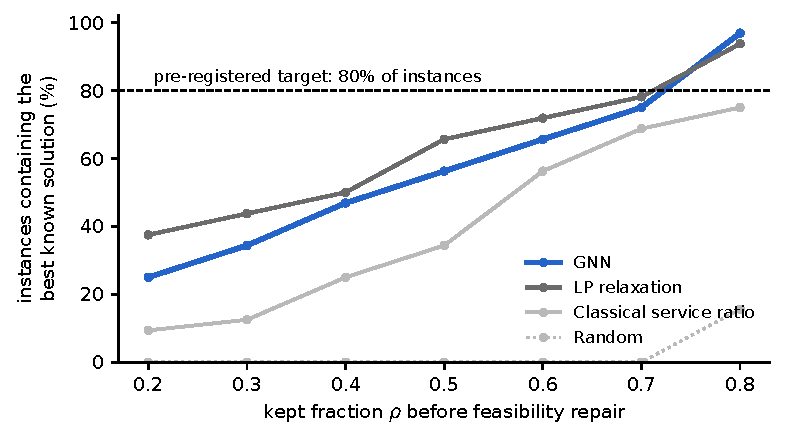
\includegraphics[width=0.92\linewidth]{../figuras/rho.pdf}
\caption{Pruning safety on the 32 validation instances (30 candidate facilities, 150 customers).
Each ranker orders the facilities; the restricted problem keeps the best-ranked fraction $\rho$
(horizontal axis) and a feasibility repair then adds facilities until a first-fit-decreasing
packing of all demands fits and every customer has one of its five cheapest facilities (the
repair alone keeps at least 41\% of the facilities, so small $\rho$ values do not mean small
restricted problems). The vertical axis is the percentage of instances whose restricted problem
still contains \emph{every} facility open in the best known solution, i.e., the percentage in
which pruning has not excluded that solution; higher is safer. The dashed line is the
pre-registered target of 80\%. \emph{GNN}: bipartite graph neural network of
Section~\ref{sec:gnn} (seed 0). \emph{LP relaxation}: facilities ordered by their opening value
$y_i$ in the strong LP. \emph{Classical service ratio}: $(f_i + \text{cost of serving its cheapest
customers up to } Q_i)$ divided by the served demand, the criterion of the greedy add heuristic.
\emph{Random}: uniform order. Source: \texttt{results/pesquisa/etapa1/rho\_validacao.csv}.}
\label{fig:rho}
\end{figure}

\subsection{Coordination is necessary}\label{sec:res-decomp}
Solving clusters independently (Section~\ref{sec:problem}) produced a capacity-infeasible union
in every examined validation instance, with 690--1{,}070 units of overload; after greedy repair
the solutions were 19--29\% above the reference. In the validation pilot, the naive decomposition
had a primal integral of 0.497 and a median final deviation of 28.8\%, against 0.024--0.041 and
1.2--2.7\% for the coordinated CLNS. The naive decomposition was not
carried to the closed test.

\subsection{Validation pilots (not the closed test)}\label{sec:res-pilot}
A first pilot (16 validation instances, one seed) motivated the hybrid. The adaptive expansion had
the lowest primal integral (0.020) and final deviation (0.3\%). CLNS variants found good solutions
early (primal integral 0.024--0.041, against 0.062--0.074 for SCIP and LNS) but stalled at
1.2--2.7\% above the best. The learned selector was the best CLNS selector but did not separate
from rotation (wins on 62\% of the instances, $p=0.43$). Figure~\ref{fig:pilot1} shows both
metrics.

\begin{figure}[t]\centering
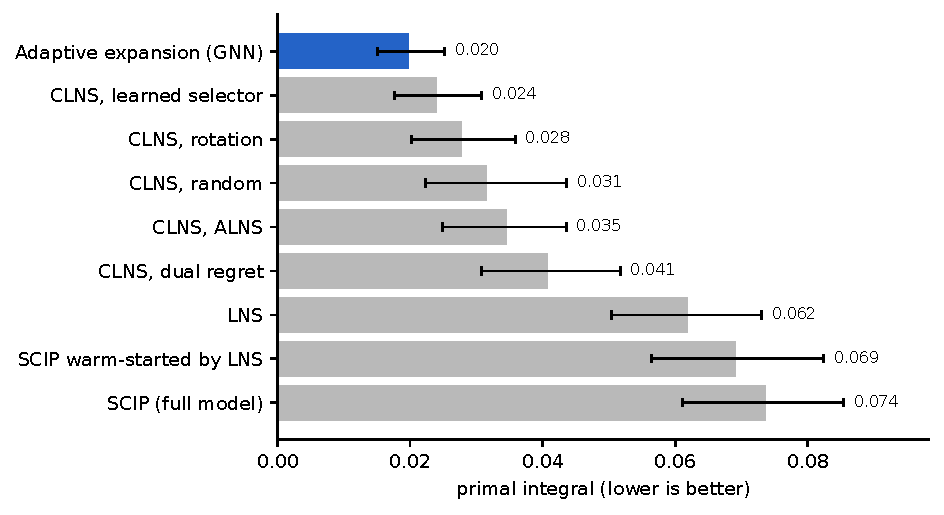
\includegraphics[width=0.49\linewidth]{../figuras/piloto1_integral.pdf}\hfill
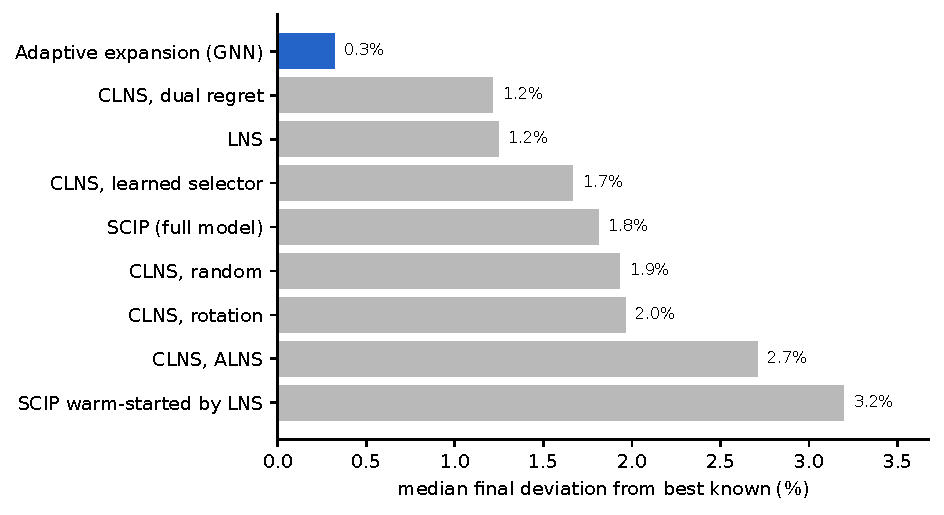
\includegraphics[width=0.49\linewidth]{../figuras/piloto1_desvio.pdf}
\caption{First validation pilot: 16 instances ($30\times150$), budget $T=60$~s, one solver seed
per method. \emph{Left, primal integral} $P = \frac{1}{T}\int_0^T g(t)\,dt$, where
$g(t) = \min\{1, (z^\ast(t) - z_{\mathrm{BKS}})/z_{\mathrm{BKS}}\}$, $z^\ast(t)$ is the best
solution found by time $t$ (with $g(t)=1$ before the first solution) and $z_{\mathrm{BKS}}$ is the
best known cost of the instance (the minimum over all methods and the reference label). $P=0$
means the best known solution was available from time zero; $P=1$ means no solution during the
whole budget. It rewards finding good solutions \emph{early}, not only ending well; lower is
better. Bars are means over instances; whiskers are 95\% bootstrap confidence intervals of the
mean (4{,}000 resamples of instances). \emph{Right, median final deviation}
$(z_{\mathrm{final}} - z_{\mathrm{BKS}})/z_{\mathrm{BKS}}$ at $T$, in percent; lower is better.
The naive decomposition (primal integral 0.497, deviation 28.8\%) is omitted to keep the scale
readable. Highlighted: the method with the lowest primal integral. Source:
\texttt{results/pesquisa/clns/81dbbcb06942419706f3}.}
\label{fig:pilot1}
\end{figure}

\paragraph{Second pilot: the hybrid.} The second pilot used the same 16 instances with three
solver seeds for stochastic methods (432 runs) under the timing protocol of
Section~\ref{sec:protocol}. Two hypotheses were registered beforehand: (H-a) the hybrid with the
GNN-guided selector has a lower primal integral than the adaptive expansion alone; (H-b) inside
the hybrid, the GNN-guided selector beats rotation and the learned selector.
Table~\ref{tab:pilot2} and Figures~\ref{fig:pilot2}--\ref{fig:pilot2-wins} report the outcome.

\begin{table}[t]\centering\small
\caption{Second validation pilot (16 instances, $30\times150$, $T=60$~s; seeds averaged within
instance). $P$: mean primal integral \eqref{eq:pi} with 95\% bootstrap interval; \emph{Dev.}:
median final deviation $g(T)$; $\le1\%$ and $\le0.1\%$: share of instances whose final deviation
is within that tolerance; \emph{Best}: share of instances in which the method has the lowest
final deviation (ties counted for all). Rows sorted by $P$.}\label{tab:pilot2}
\resizebox{\linewidth}{!}{%
\begin{tabular}{lcrrrr}
\toprule
Method & $P$ (95\% CI) & Dev. (\%) & $\le1\%$ & $\le0.1\%$ & Best \\
\midrule
Adaptive expansion (GNN) & 0.0257 (0.019--0.035) & 0.81 & 62.5 & 12.5 & 25.0 \\
Hybrid, learned selector & 0.0270 (0.020--0.036) & 0.57 & 87.5 & 6.3 & 12.5 \\
Hybrid, rotation & 0.0274 (0.021--0.035) & 0.63 & 62.5 & 18.8 & 25.0 \\
CLNS, learned selector & 0.0292 (0.023--0.036) & 2.12 & 12.5 & 0.0 & 6.3 \\
Hybrid, GNN-guided & 0.0296 (0.022--0.040) & 0.62 & 68.8 & 12.5 & 25.0 \\
CLNS, ALNS & 0.0337 (0.029--0.038) & 2.40 & 12.5 & 0.0 & 0.0 \\
CLNS, rotation & 0.0359 (0.030--0.043) & 2.31 & 18.8 & 0.0 & 6.3 \\
CLNS, GNN-guided & 0.0423 (0.034--0.051) & 1.88 & 0.0 & 0.0 & 6.3 \\
LNS & 0.0700 (0.059--0.082) & 1.84 & 12.5 & 0.0 & 0.0 \\
SCIP warm-started by LNS & 0.0705 (0.059--0.084) & 3.59 & 25.0 & 0.0 & 0.0 \\
SCIP (full model) & 0.0795 (0.067--0.091) & 2.66 & 18.8 & 12.5 & 12.5 \\
\bottomrule
\end{tabular}}
\end{table}

Neither hypothesis was supported. (H-a) The adaptive expansion alone has the lowest primal
integral (0.0257); the three hybrids are within its confidence interval (0.0270--0.0296) but not
below it. What the hybrid changes is the \emph{end} of the run: its median final deviation is
0.57--0.63\% against 0.81\%, and with the learned selector 87.5\% of the instances finish within
1\% of the best known solution, against 62.5\%. The anytime curves (Figure~\ref{fig:pilot2},
right) are consistent with this: after $\alpha T=30$~s the expansion flattens near 0.8\%, while
the CLNS phase keeps improving. The two curves need not coincide before $\alpha T$, and they do
not (2.8\% against 3.5\% at 5~s), because the expansion alone allots its stages from a budget of
$T$ and the hybrid from $\alpha T$. The primal integral, dominated by the first seconds, barely
registers the late gain. (H-b) Inside the hybrid, the GNN-guided selector (0.0296) is not better than
rotation (0.0274) or the learned selector (0.0270); the differences are far smaller than the
intervals. The facility scores help in ordering the facilities for the expansion, but once a
good solution exists they carry no measurable information about \emph{where} to search next.

Two further observations hold across both pilots. First, every method that restricts the search
space dominates SCIP on the full model in primal integral by a factor of 2--3, and the hybrids have a lower final deviation in 13--14 of 16 instances (Figure~\ref{fig:pilot2-wins}). Second, CLNS
without the expansion stalls at about 2\%, regardless of the selector: one hypothesis, not tested here, is
that from the LP-rounded solution the improving moves require opening and closing several
facilities at once, which the five neighborhoods rarely free together. This is the motivation for the controls of
Section~\ref{sec:res-controls}: if neither the GNN nor the learned selector separates from its
learning-free counterpart, the gain may come from the mechanisms (nested restriction,
coordinated subproblems) rather than from learning.

\begin{figure}[t]\centering
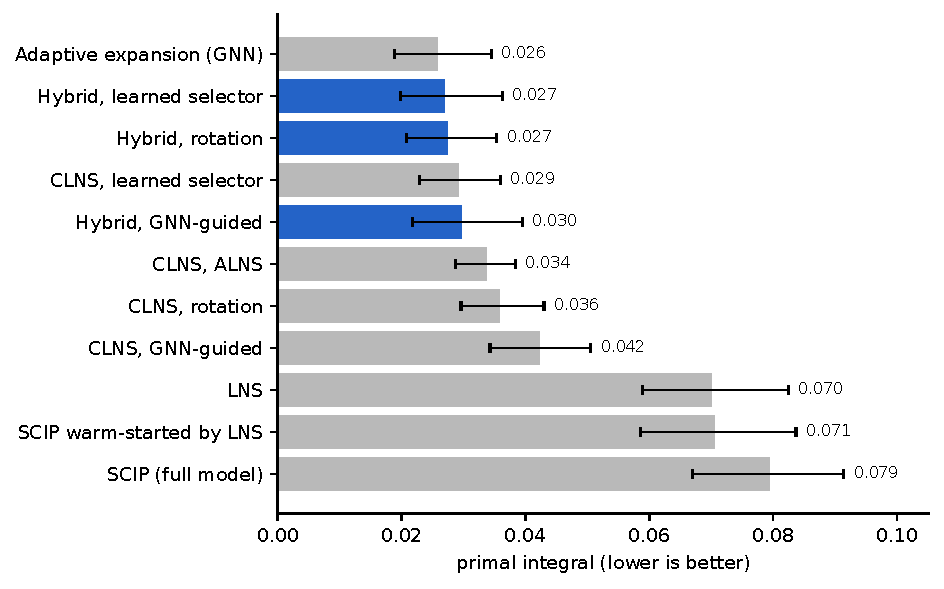
\includegraphics[width=0.49\linewidth]{../figuras/piloto2_integral.pdf}\hfill
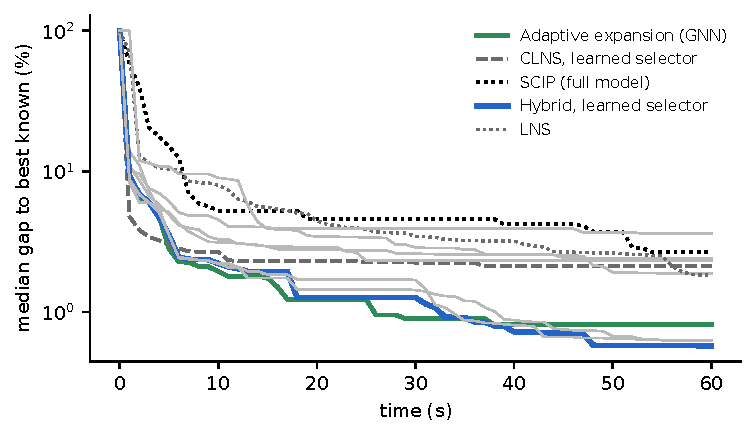
\includegraphics[width=0.49\linewidth]{../figuras/piloto2_anytime.pdf}
\caption{Second validation pilot (16 instances, $30\times150$, $T=60$~s, three seeds averaged
within instance). \emph{Left}: mean primal integral $P$ \eqref{eq:pi} per method; whiskers are
95\% bootstrap confidence intervals over instances; the three hybrids are highlighted; lower is
better. The whiskers are marginal intervals; paired comparisons are given in the text.
\emph{Right}: anytime behaviour. For each second $t$ of the budget, the curve is the median over
instances of the primal gap $g(t)$ in percent (logarithmic vertical axis; a value of $10^0$ is a
1\% gap). A curve that drops early and stays low has a small primal integral; a curve that keeps
dropping late has a small final deviation. Highlighted: hybrid with the learned selector (blue),
adaptive expansion (green), CLNS with the learned selector (dashed), SCIP on the full model
(dotted black) and LNS (dotted grey); the remaining methods are drawn in light grey for context.
Source: \texttt{results/pesquisa/clns/eaa3f86d9312c0970ce9/agregados.json}.}
\label{fig:pilot2}
\end{figure}

\begin{figure}[t]\centering
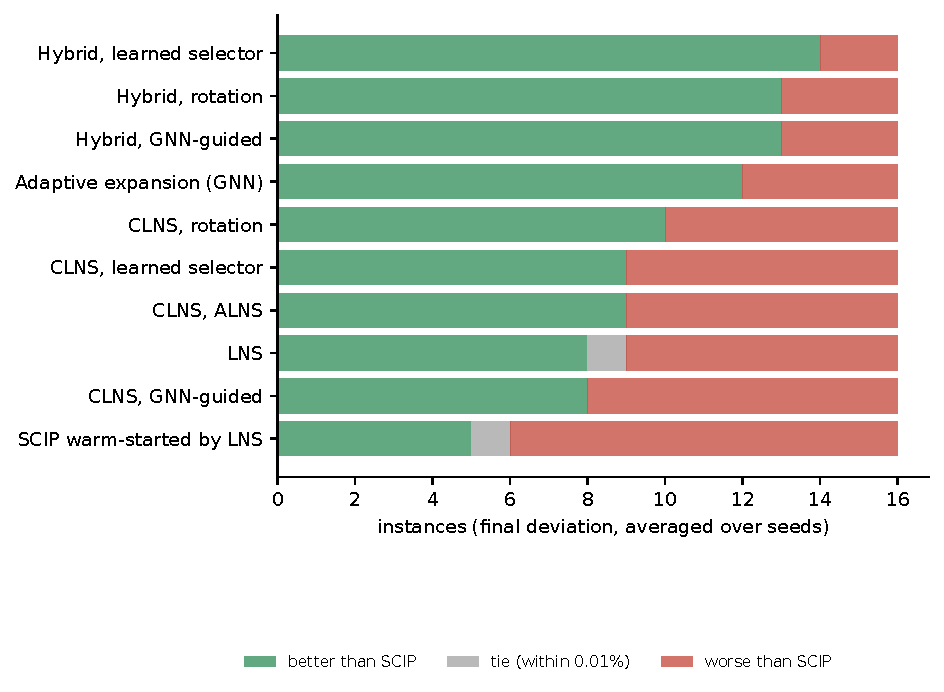
\includegraphics[width=0.49\linewidth]{../figuras/piloto2_vitorias.pdf}\hfill
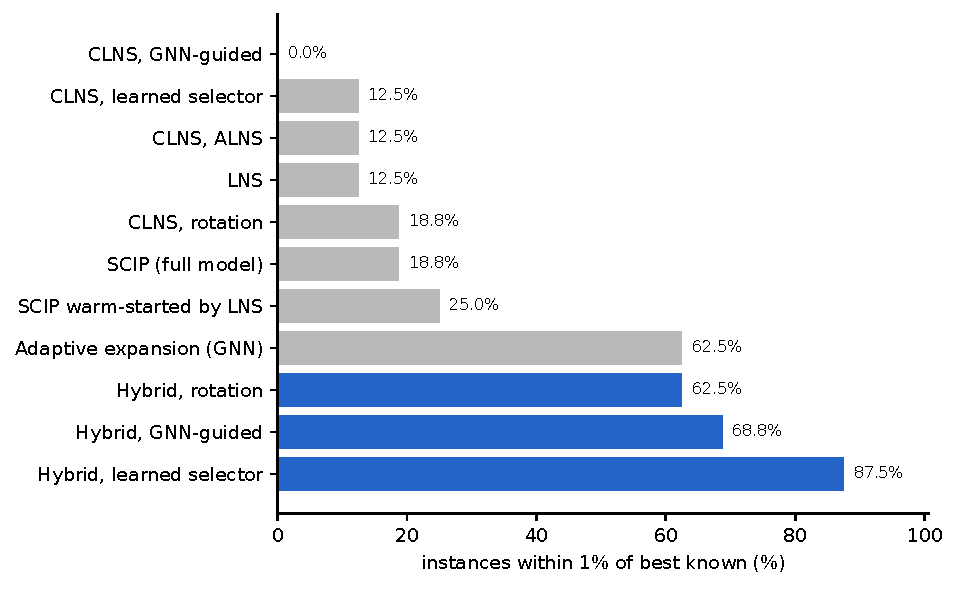
\includegraphics[width=0.49\linewidth]{../figuras/piloto2_ate1pct.pdf}
\caption{Second validation pilot, paired and threshold views. \emph{Left}: for each method, the
number of the 16 instances in which its final deviation (seeds averaged) is lower than
(green), equal within $10^{-4}$ to (grey) or higher than (red) that of SCIP on the full model.
This is a descriptive count; it does not depend on the magnitude of the differences, which the
Wilcoxon test does use. \emph{Right}: percentage of instances whose final deviation is at most 1\%; hybrids
highlighted; higher is better. Same source as Figure~\ref{fig:pilot2}.}
\label{fig:pilot2-wins}
\end{figure}

\subsection{Is learning necessary? Classical controls and subproblem memory}\label{sec:res-controls}
The third pilot used the same 16 validation instances, budget and protocol (352 runs), with the
corrected CLNS code, and added the learning-free controls of Sections~\ref{sec:expansion} and
\ref{sec:kernel} and the memory of Section~\ref{sec:memory}. It answers two questions: does the
GNN matter, and does remembering failed subproblems help? Since it re-ran SCIP, the GNN expansion,
CLNS and the hybrid with rotation, it also checks the second pilot under the corrected code: the
picture is unchanged (hybrid and expansion tied, CLNS alone behind them, SCIP last).

\begin{table}[t]\centering\small
\caption{Third validation pilot (16 instances, $30\times150$, $T=60$~s; seeds averaged within
instance). Columns as in Table~\ref{tab:pilot2}. \emph{Learned}: whether any component of the
method was trained. Rows sorted by $P$.}\label{tab:pilot3}
\resizebox{\linewidth}{!}{%
\begin{tabular}{lccrrrr}
\toprule
Method & Learned & $P$ (95\% CI) & Dev. (\%) & $\le1\%$ & $\le0.1\%$ & Best \\
\midrule
Adaptive expansion (LP) & no & 0.0192 (0.015--0.024) & 0.17 & 56.3 & 43.8 & 31.3 \\
LP hybrid, rotation & no & 0.0215 (0.017--0.026) & 0.53 & 75.0 & 18.8 & 31.3 \\
LP hybrid, rotation + memory & no & 0.0217 (0.017--0.027) & 0.59 & 87.5 & 18.8 & 31.3 \\
Hybrid (GNN), rotation & yes & 0.0236 (0.019--0.028) & 0.87 & 68.8 & 12.5 & 6.3 \\
Hybrid (GNN), rotation + memory & yes & 0.0238 (0.019--0.029) & 0.87 & 68.8 & 12.5 & 12.5 \\
Adaptive expansion (GNN) & yes & 0.0240 (0.018--0.030) & 0.93 & 50.0 & 12.5 & 12.5 \\
Kernel search & no & 0.0258 (0.019--0.033) & 0.99 & 56.3 & 12.5 & 18.8 \\
CLNS, rotation + memory & no & 0.0347 (0.031--0.039) & 2.36 & 0.0 & 0.0 & 0.0 \\
CLNS, rotation & no & 0.0372 (0.032--0.043) & 2.80 & 0.0 & 0.0 & 0.0 \\
SCIP (full model) & no & 0.0706 (0.060--0.081) & 2.44 & 18.8 & 6.3 & 6.3 \\
\bottomrule
\end{tabular}}
\end{table}

\paragraph{No evidence of a benefit from the GNN.} Replacing the GNN score by the LP score \eqref{eq:lpscore},
which requires no training data, did not worsen any method and numerically improved all of them
(Table~\ref{tab:pilot3}, Figure~\ref{fig:pilot3}). For the adaptive expansion, the LP score gave
a primal integral of 0.0192 against 0.0240 and a median final deviation of 0.17\% against 0.93\%;
it had the lower primal integral in 11 of the 16 instances (paired Wilcoxon $p=0.13$). For the
hybrid, 0.0215 against 0.0236 (lower in 10 of 16, $p=0.43$). With 16 instances none of these
differences is significant, so the supported statement is the weaker one: \emph{there is no
evidence that the learned score helps}, and the point estimates favor the learning-free score.
This is consistent with Section~\ref{sec:res-pruning}, where the LP ranking was at least as safe
as the GNN for pruning. Kernel search, the established classical method, is at the level of the
GNN expansion (0.0258 against 0.0240; $p=0.16$ against the LP expansion) and beats SCIP on the
full model in 14 of 16 instances. The reduced-cost certificate \eqref{eq:cert} closed one of the
16 instances before the last stage for both scores.

\paragraph{What the CLNS phase adds.} With the LP score, the hybrid does not improve the primal
integral of the expansion alone (0.0215 against 0.0192, $p=0.40$). Its effect on the end of the
run is mixed: more instances finish within 1\% (75.0\% against 56.3\%) and the mean final
deviation is lower by 0.16 percentage points, but fewer finish within 0.1\% (18.8\% against
43.8\%) and the median deviation is higher (0.53\% against 0.17\%). The expansion, given the
whole budget, closes or nearly closes the easier instances; the hybrid, which stops the
expansion at $\alpha T$, trades those for more robust results on the harder ones. The choice of
$\alpha$ therefore matters and is part of the ablations.

\paragraph{Subproblem repetition and memory.} Without memory, 54--58\% of the subproblems
selected by the CLNS had already failed from the same local state with at least the same time
limit (Figure~\ref{fig:pilot3-mem}): more than half of the iterations re-ran a mixed-integer
program that had already been tried without success under at least the same limit. Memory removed about half of these; the remaining
25--27\% are iterations in which \emph{every} generated candidate had already failed under the
current limit. This is not a certificate of local optimality: the subproblems were interrupted,
not solved, and the candidate list is a sample of the neighborhoods. The time freed by memory did
not translate into a measurable gain: for CLNS alone the primal integral went from 0.0372 to
0.0347 ($p=0.18$) and the median deviation from 2.80\% to 2.36\% ($p=0.12$); inside the hybrids
there was no change (differences below 0.0003 in $P$). One reading, compatible with these data but not established by them, is that the CLNS is limited
by the \emph{reach} of its neighborhoods (or by the ten-facility candidate restriction, or by the
short limits) more than by the order in which they are tried. Re-solving a sample of repeated
subproblems with larger limits would separate these explanations and is listed as future work.

\begin{figure}[t]\centering
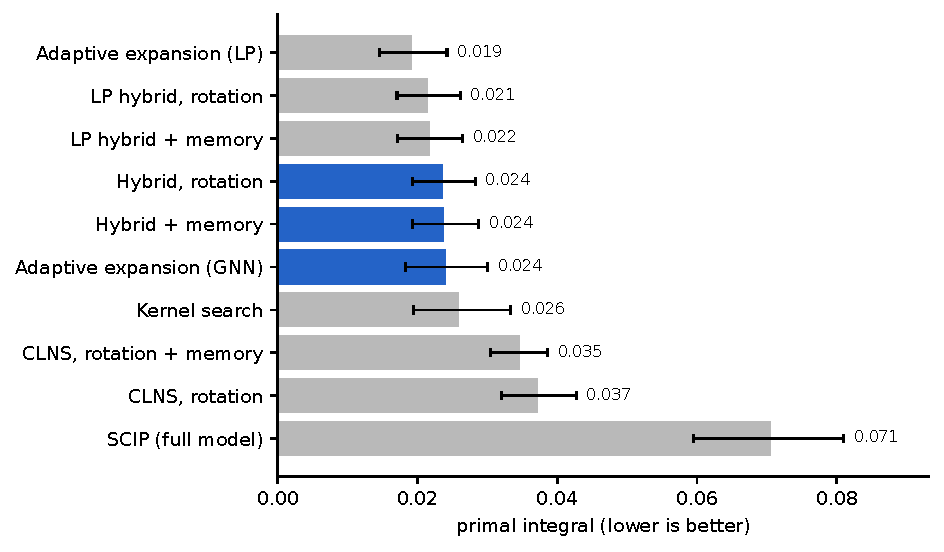
\includegraphics[width=0.49\linewidth]{../figuras/piloto3_integral.pdf}\hfill
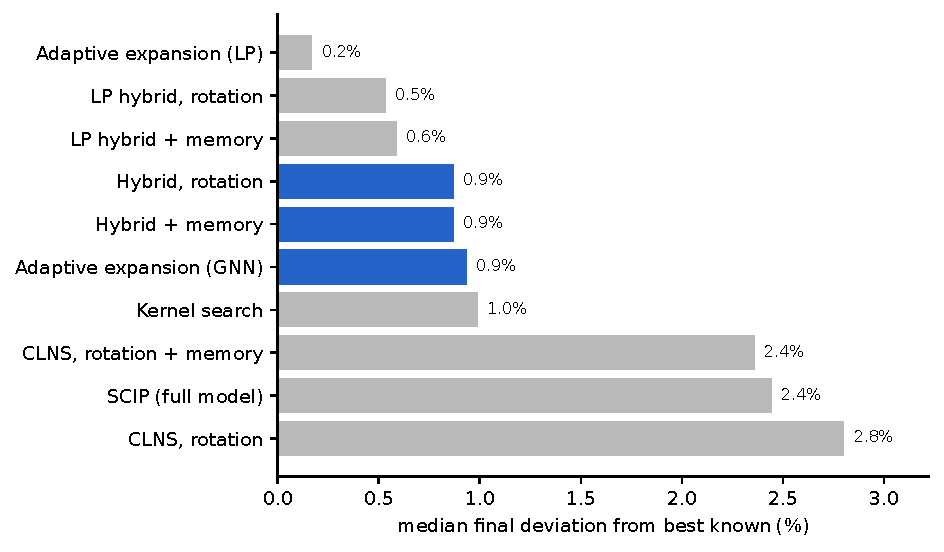
\includegraphics[width=0.49\linewidth]{../figuras/piloto3_desvio.pdf}
\caption{Third validation pilot (16 instances, $30\times150$, $T=60$~s; seeds averaged within
instance). \emph{Left}: mean primal integral $P$ \eqref{eq:pi}; whiskers are 95\% bootstrap
confidence intervals over instances. \emph{Right}: median final deviation $g(T)$ in percent. In
both panels lower is better and the highlighted bars are the methods with a learned component
(the GNN score); grey bars use no training. ``LP'' denotes the score \eqref{eq:lpscore} computed
from the strong LP relaxation. Source:
\texttt{results/pesquisa/clns/e1a72d506f53ea707aa1/agregados.json}.}
\label{fig:pilot3}
\end{figure}

\begin{figure}[t]\centering
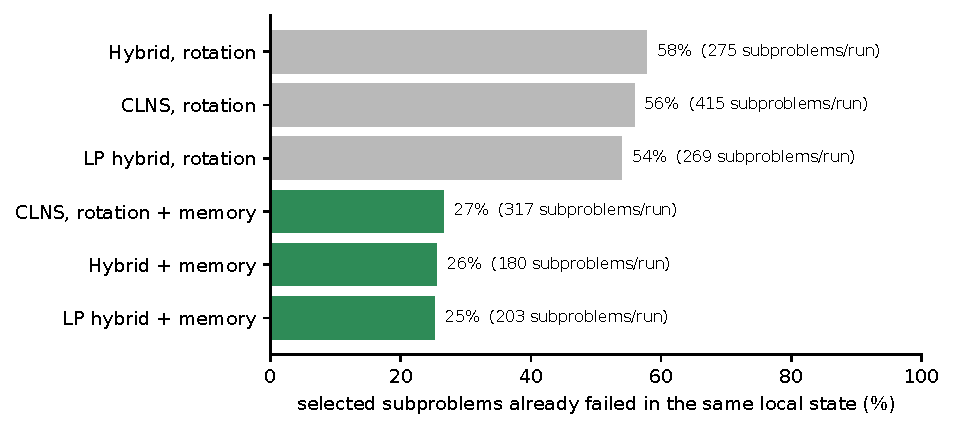
\includegraphics[width=0.7\linewidth]{../figuras/piloto3_repeticao.pdf}
\caption{Repetition of subproblems in the third pilot. For each CLNS variant, the bar is the
percentage of iterations in which the selected subproblem had the same key \eqref{eq:key} as a
subproblem that had already failed to improve with a time limit at least as large, averaged over
seeds and then over instances. Green bars have the memory enabled; for them the remaining
repetitions are iterations in which all candidates were exhausted. The label gives the mean
number of subproblems solved per run; with memory it is lower, plausibly because the subproblems
that remain are those the solver has not yet answered, which take longer. Source:
\texttt{results/pesquisa/clns/e1a72d506f53ea707aa1/resultados.csv}.}
\label{fig:pilot3-mem}
\end{figure}

\paragraph{Measurement.} In this pilot the median CPU/wall ratio was 0.999 and seven of the 352
runs (2.0\%) were below 0.9, all on the same core; the 95th percentile of the budget overrun was
0.04~s.

\subsection{Closed test}\label{sec:res-test}
The closed test was pre-registered after the third pilot and before any run on the instances
below: the six methods, the budgets, four hypotheses and the analysis script were committed
first. It comprises 1{,}390 runs on 139 instances that no pilot had used. The hypotheses are
evaluated on the 64 synthetic instances (test, corridor and scale) with the paired Wilcoxon
signed-rank test and Holm's correction over the four hypotheses, separately for the primal
integral (primary) and the final deviation (secondary):
\begin{description}
\item[H1] restriction helps: the LP-ranked adaptive expansion differs from SCIP on the full model;
\item[H2] learning: the GNN-ranked expansion differs from the LP-ranked expansion;
\item[H3] the CLNS phase: the LP hybrid differs from the LP-ranked expansion alone;
\item[H4] the established classical method: the LP-ranked expansion differs from kernel search.
\end{description}

\begin{table}[t]\centering\small
\caption{Closed test, synthetic sets. $P$: mean primal integral \eqref{eq:pi} with 95\% bootstrap
interval over instances; \emph{Dev.}: median final deviation $g(T)$ from the best known solution;
$\le1\%$: share of instances finishing within 1\%; \emph{W/T/L}: instances in which the final
deviation is lower than, equal to (within $10^{-4}$) or higher than that of SCIP on the full
model. Seeds averaged within instance. Rows sorted by $P$ on the pooled set.}\label{tab:closed}
\resizebox{\linewidth}{!}{%
\begin{tabular}{l rr rr rr | crrc}
\toprule
 & \multicolumn{2}{c}{Test (32, 60 s)} & \multicolumn{2}{c}{Corridor (16, 60 s)} &
 \multicolumn{2}{c|}{Scale (16, 120 s)} & \multicolumn{4}{c}{Pooled (64)} \\
Method & $P$ & Dev. & $P$ & Dev. & $P$ & Dev. & $P$ (95\% CI) & Dev. & $\le1\%$ & W/T/L \\
\midrule
LP hybrid & 0.0385 & 0.35 & 0.0289 & 0.23 & 0.0621 & 0.58 & 0.0420 (0.032--0.053) & 0.35 & 70.3 & 54/3/7 \\
Kernel search & 0.0364 & 0.81 & 0.0341 & 0.85 & 0.0616 & 0.52 & 0.0422 (0.032--0.055) & 0.74 & 57.8 & 46/6/12 \\
Adaptive expansion (LP) & 0.0412 & 0.29 & 0.0311 & 0.73 & 0.0854 & 0.44 & 0.0497 (0.033--0.070) & 0.50 & 65.6 & 50/7/7 \\
Hybrid (GNN) & 0.0506 & 0.55 & 0.0423 & 0.18 & 0.1275 & 2.19 & 0.0677 (0.051--0.087) & 0.62 & 59.4 & 53/3/8 \\
Adaptive expansion (GNN) & 0.0659 & 0.90 & 0.0540 & 0.15 & 0.1699 & 2.03 & 0.0889 (0.058--0.124) & 0.64 & 56.3 & 42/9/13 \\
SCIP (full model) & 0.0794 & 3.21 & 0.1057 & 3.59 & 0.1688 & 7.00 & 0.1083 (0.093--0.124) & 3.72 & 23.4 & -- \\
\bottomrule
\end{tabular}}
\end{table}

\begin{table}[t]\centering\small
\caption{Pre-registered hypotheses on the pooled synthetic set (64 instances). $\bar\Delta$: mean
of the per-instance difference A~$-$~B, with 95\% bootstrap interval; negative values favor A.
The deviation is in percentage points. \emph{A/B}: number of instances in which A or B is
better. $p$: paired Wilcoxon signed-rank test; $p_{\mathrm{Holm}}$: after Holm's correction over
the four hypotheses of the same metric.}\label{tab:hyp}
\resizebox{\linewidth}{!}{%
\begin{tabular}{lll rcrr rcrr}
\toprule
 & & & \multicolumn{4}{c}{Primal integral} & \multicolumn{4}{c}{Final deviation (p.p.)} \\
 & A & B & $\bar\Delta$ (95\% CI) & A/B & $p$ & $p_{\mathrm{Holm}}$ & $\bar\Delta$ (95\% CI) & A/B & $p$ & $p_{\mathrm{Holm}}$ \\
\midrule
H1 & expansion (LP) & SCIP & $-0.059$ ($-0.084$, $-0.031$) & 55/9 & $<0.001$ & $<0.001$ & $-3.10$ ($-4.07$, $-2.18$) & 50/7 & $<0.001$ & $<0.001$ \\
H2 & expansion (GNN) & expansion (LP) & $+0.039$ ($+0.014$, $+0.071$) & 22/42 & 0.001 & 0.004 & $+0.57$ ($+0.14$, $+1.05$) & 15/32 & 0.014 & 0.043 \\
H3 & LP hybrid & expansion (LP) & $-0.008$ ($-0.018$, $+0.001$) & 31/33 & 0.659 & 0.659 & $-0.54$ ($-1.06$, $-0.12$) & 38/19 & 0.025 & 0.050 \\
H4 & expansion (LP) & kernel search & $+0.008$ ($-0.001$, $+0.018$) & 36/28 & 0.319 & 0.638 & $-0.32$ ($-0.69$, $+0.03$) & 33/20 & 0.050 & 0.050 \\
\bottomrule
\end{tabular}}
\end{table}

Tables~\ref{tab:closed} and~\ref{tab:hyp} and Figures~\ref{fig:closed}--\ref{fig:closed-hyp}
give the outcome.

\paragraph{H1: restriction helps.} The LP-ranked expansion has less than half the primal integral
of SCIP on the full model (0.050 against 0.108) and a median final deviation of 0.50\% against
3.72\%; it is better in 55 of the 64 instances ($p_{\mathrm{Holm}}<0.001$ for both metrics).
Every restriction-based method beats the full model in at least 42 instances.

\paragraph{H2: the learned ranking is worse than the LP ranking.} The pilots could only say that
there was no evidence in favor of the GNN. The closed test is stronger: with the GNN in place of
the LP score, the primal integral of the expansion rises from 0.050 to 0.089
($\bar\Delta=+0.039$, interval $+0.014$ to $+0.071$, LP better in 42 of 64,
$p_{\mathrm{Holm}}=0.004$) and the mean final deviation rises by 0.57 percentage points
($p_{\mathrm{Holm}}=0.043$). The loss grows with the distance from the training distribution: on
the scale set, twice as large as anything the GNN was trained on, the GNN-ranked expansion
(0.170) is no better than SCIP on the full model (0.169), whereas the LP-ranked one stays at
0.085. On the corridor family, never seen in training, the GNN variants end with the lowest
\emph{median} deviations (0.15--0.18\%) but have higher primal integrals than their LP
counterparts, so the learned ranking is not uniformly worse at the end of the run; it is slower
to get there. The LP score needs no training data and adapts to each instance by construction.

\paragraph{H3: the CLNS phase improves where the search ends, not how fast it gets there.}
Adding the CLNS phase to the LP-ranked expansion leaves the primal integral unchanged (0.042
against 0.050, $p_{\mathrm{Holm}}=0.66$) and lowers the final deviation by 0.54 percentage
points on average (interval $-1.06$ to $-0.12$; better in 38 instances, worse in 19). The
corrected $p$-value is 0.0495, at the threshold, so we regard this as suggestive rather than
established. The hybrid has the lowest pooled primal integral and the highest share of instances
within 1\% (70.3\%).

\paragraph{H4: the nested expansion is at the level of kernel search.} The two do not differ in
primal integral ($p_{\mathrm{Holm}}=0.64$; kernel search is numerically lower, 0.042 against
0.050). In final deviation the expansion is lower by 0.32 points with an interval that includes
zero ($-0.69$ to $+0.03$) and a corrected $p$-value of 0.0495. We do not claim a difference.
Kernel search, published in 2014 and using no learning, has a numerically lower primal
integral than both learned variants (0.042 against 0.068 and 0.089).

\begin{figure}[t]\centering
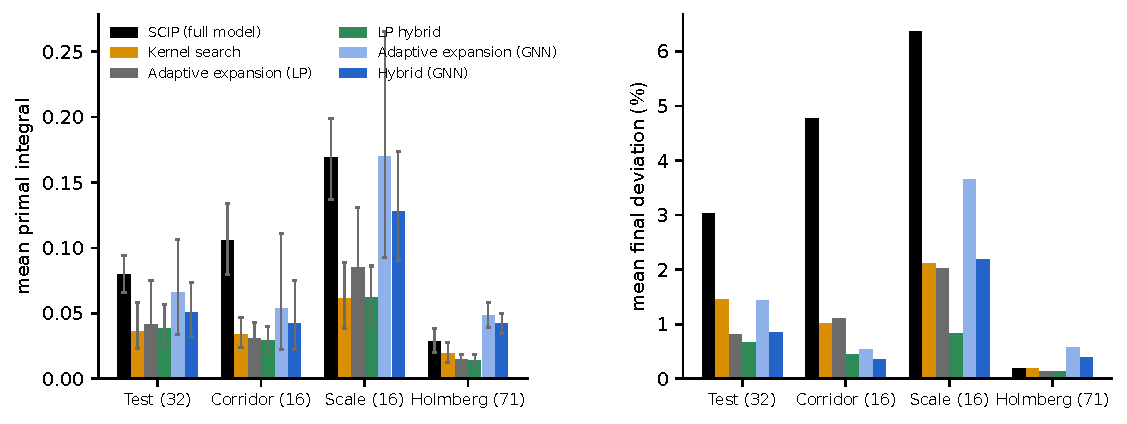
\includegraphics[width=\linewidth]{../figuras/fechado_conjuntos.pdf}
\caption{Closed test, by instance set (number of instances in parentheses). \emph{Left}: mean
primal integral $P$ \eqref{eq:pi}; whiskers are 95\% bootstrap intervals over instances; lower is
better. \emph{Right}: mean final deviation $g(T)$ in percent (from the published optimum for
Holmberg, from the best known solution otherwise). Black: SCIP on the full model. Orange: kernel
search. Grey and green: LP-ranked expansion and LP hybrid, which use no learning. Light and dark
blue: their GNN-ranked counterparts. Within each set the two blue bars are to be compared with the
grey and green ones: the difference is the effect of replacing the LP score by the learned one.
Source: \texttt{results/pesquisa/fechado/analise.json}.}
\label{fig:closed}
\end{figure}

\begin{figure}[t]\centering
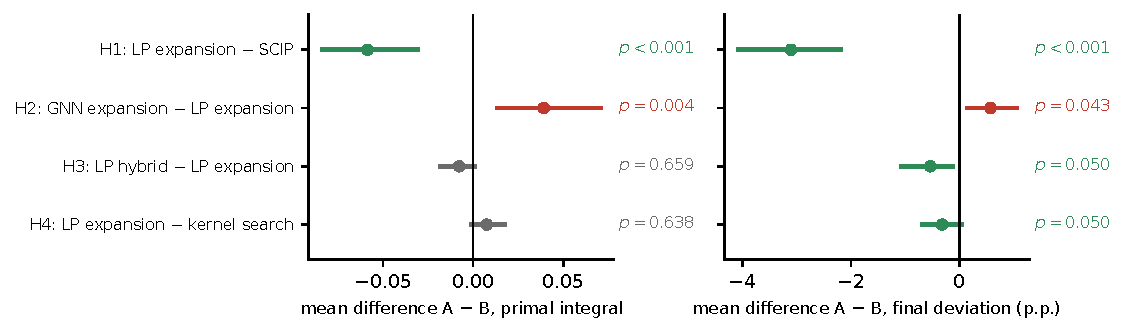
\includegraphics[width=\linewidth]{../figuras/fechado_hipoteses.pdf}
\caption{Pre-registered hypotheses on the 64 pooled synthetic instances. Each row is one paired
comparison A~$-$~B: the dot is the mean per-instance difference and the bar its 95\% bootstrap
interval; a bar entirely to the left of zero means that A is better. \emph{Left}: primal
integral. \emph{Right}: final deviation in percentage points. The value at the right of each row
is the Holm-corrected Wilcoxon $p$-value. Green: significant in favor of A; red: significant in
favor of B; grey: not significant at 0.05.}
\label{fig:closed-hyp}
\end{figure}

\subsection{External anchor: Holmberg instances}\label{sec:res-holmberg}
The 71 Holmberg instances have published optima, so deviations here are true optimality gaps
(Table~\ref{tab:holmberg}). They are small by current standards: SCIP on the full model reaches
the optimum in 61 of them within 30~s, with a median run time of 1.2~s. Three observations hold.
First, the reduced-cost certificate \eqref{eq:cert} works as intended: the expansion stopped with
a \emph{proven} global optimum before its last stage in 59 of the 71 instances, with either
ranking, and with the LP ranking it did so in a median of 0.9~s. Second, the LP-ranked expansion
matches the full model in the number of optima (61) with half its primal integral (0.015 against
0.029). Third, the GNN, trained on Euclidean instances with 30 facilities, transfers poorly to
these non-Euclidean instances: its variants have the highest primal integrals (0.042--0.048),
above the full model, and their certified runs take a median of 4.5~s against 0.9~s, a
difference we attribute to computing the features and the learned score.

\begin{table}[t]\centering\small
\caption{Holmberg instances (71, $T=30$~s). $P$: mean primal integral with 95\% bootstrap
interval; \emph{Mean dev.}: mean deviation from the published optimum; \emph{Optimum}: instances
in which the published optimum was reached (in every seed); \emph{Certified}: instances in which
the expansion proved optimality by reduced costs before its last stage.}\label{tab:holmberg}
\resizebox{\linewidth}{!}{%
\begin{tabular}{lcrrr}
\toprule
Method & $P$ (95\% CI) & Mean dev. (\%) & Optimum & Certified \\
\midrule
LP hybrid & 0.0143 (0.011--0.018) & 0.13 & 59 & -- \\
Adaptive expansion (LP) & 0.0146 (0.011--0.018) & 0.14 & 61 & 59 \\
Kernel search & 0.0191 (0.012--0.028) & 0.18 & 60 & -- \\
SCIP (full model) & 0.0286 (0.020--0.039) & 0.20 & 61 & -- \\
Hybrid (GNN) & 0.0419 (0.035--0.050) & 0.39 & 53 & -- \\
Adaptive expansion (GNN) & 0.0481 (0.039--0.058) & 0.57 & 59 & 59 \\
\bottomrule
\end{tabular}}
\end{table}

\subsection{Case study: Olist}\label{sec:res-olist}
The four real instances grow from $30\times150$ to $150\times850$ and are reported descriptively
(Table~\ref{tab:olist}); four instances support no statistical claim. They show a regime that
the synthetic sets do not reach. On the two largest instances, SCIP on the full model, kernel
search and the expansion alone ended at the same solutions, 8.7--9.3\% above the best known,
and on the largest the expansion returned no feasible solution within 120~s. The hybrids,
whose CLNS phase starts from the LP-rounded solution when the expansion returns nothing, finished
0.02--0.15\% from the best known solution. When the full model no longer fits in the budget,
coordinated decomposition is not a refinement but the only component that makes progress. On the
smallest instance the order is reversed: the full model is already within 0.06\% and the hybrids,
which stop the exact search at $\alpha T$, end slightly behind.

\begin{table}[t]\centering\small
\caption{Olist instances ($T=120$~s): final deviation from the best known solution, in percent,
averaged over seeds. ``--'': no feasible solution within the budget.}\label{tab:olist}
\begin{tabular}{lrrrr}
\toprule
Method & $30\times150$ & $60\times300$ & $100\times600$ & $150\times850$ \\
\midrule
LP hybrid & 0.26 & 1.03 & 0.10 & 0.02 \\
Hybrid (GNN) & 0.19 & 0.73 & 0.15 & 0.02 \\
Kernel search & 0.06 & 0.77 & 8.68 & 9.26 \\
SCIP (full model) & 0.06 & 3.06 & 8.68 & 9.26 \\
Adaptive expansion (LP) & 0.06 & 3.06 & 8.68 & -- \\
Adaptive expansion (GNN) & 0.06 & 3.06 & 8.68 & -- \\
\bottomrule
\end{tabular}
\end{table}

\subsection{Ablations}
\todo{$\alpha\in\{0.3,0.5,0.7\}$; without the opening subproblem; without the LP start; cluster
size 10/15/30.}

\subsection{Measurement quality}\label{sec:res-measure}
Because the comparison is by wall-clock time, a run that waits for the processor is penalized
for reasons unrelated to the algorithm. For every run we record the ratio between the CPU time
of the process and the wall-clock time; a single-threaded run that never waits has ratio 1. In
the 432 runs of the second pilot the median ratio was 0.996 (5th percentile 0.943, 1st percentile
0.911), and three runs (0.7\%) fell below the contention threshold of 0.9
(Figure~\ref{fig:cpu}). The budget overrun, i.e., wall-clock time beyond $T$ caused by
non-preemptible solver calls, had a 95th percentile of 0.075~s and a maximum of 0.82~s
(1.4\% of $T$).

\paragraph{Closed test.} The closed test was less clean than the pilots, and we report it as it
is. Two suspensions of the machine invalidated six runs of the test set (wall-clock times of 646
to 15{,}386~s with a CPU/wall ratio below 0.1); they were discarded by a rule based on time
alone (overrun above 60~s and ratio below 0.1), registered as a deviation before the analysis,
and re-run. More importantly, other workloads were active on the machine during the corridor and
scale sets: the median system load recorded by the harness was 86--91\%, the median CPU/wall
ratio dropped to 0.89 and 0.88, and 187 of their 320 runs fell below the 0.9 threshold. Over
all 1{,}390 runs, 229 (16.5\%) are flagged. The flags are spread over the methods in proportion
to their number of runs, so the contention slows every method rather than a particular one, and
as pre-registered all runs are kept in the main analysis. Repeating the tests of
Table~\ref{tab:hyp} without the flagged runs (38--42 instances remain per comparison) gives the
same conclusions for the primal integral: H1 ($p_{\mathrm{Holm}}<0.001$) and H2
($p_{\mathrm{Holm}}=0.006$) significant, H3 and H4 not ($p_{\mathrm{Holm}}=0.54$). Absolute
primal integrals of the corridor and scale sets should nevertheless be read as upper estimates,
and a replication of these two sets on an idle machine is listed as future work.

\begin{figure}[t]\centering
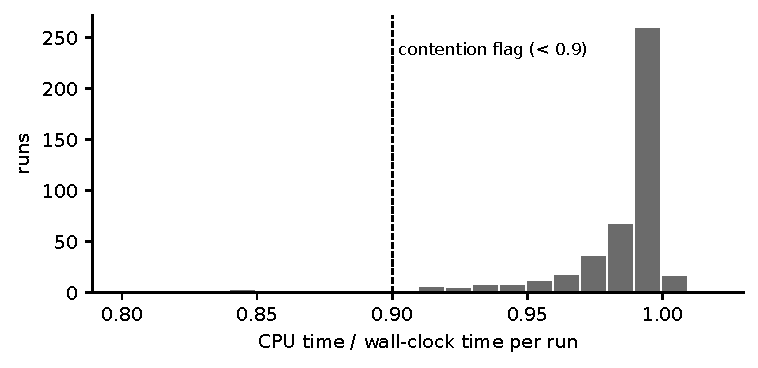
\includegraphics[width=0.7\linewidth]{../figuras/piloto2_cpu_parede.pdf}
\caption{Measurement quality in the second pilot: histogram of the ratio CPU time / wall-clock
time over the 432 runs (bins of 0.01). A ratio of 1 means the process ran without waiting for
the processor; values below the dashed line (0.9) are flagged as suspected contention and
reported, not discarded. The concentration at 0.99--1.00 indicates that pinning each run to a
dedicated physical core removed almost all interference between concurrent runs.}
\label{fig:cpu}
\end{figure}

\section{Discussion}\label{sec:discussion}

\paragraph{Guide, do not prune.}
Under capacity coupling, the information a ranking carries is better spent deciding \emph{where
to search} than \emph{what to remove}. Pruning is irreversible and has to keep slack for every
capacity constraint; guidance keeps the full domain reachable and only changes the order in which
the search visits it. This matches the trend from learned pruning towards trust regions
\citep{han2023}, learned neighborhoods \citep{huang2023} and learned delegation
\citep{li2021delegate}. \todo{confirm or revise with the closed-test result}.

\paragraph{The mechanism, not the learning.}
In the pilots the gain over the full solver came from the two restriction mechanisms, and
replacing each learned component by a learning-free one did not reduce it: the LP score in place
of the GNN, rotation in place of the learned selector. We see two reasons. The strong LP already
encodes most of what the GNN can learn about which facilities are worth opening, and it does so
for the instance at hand rather than for a training distribution. And the selector operates on a
set of neighborhoods whose joint local optimum is reached quickly: once every candidate has
failed, no ordering helps. The repetition rate we measured (54--58\% without memory, 25--27\% of
iterations fully exhausted with it) is a direct, inexpensive diagnostic of this situation, and we
suggest reporting it for any LNS before investing in a learned selector.

\paragraph{The classical counterpart is the baseline that matters.}
In every line of work we reconstructed, a classical rule with the same function captured most of
the gain: the LP ranking for pruning, the add-gain filter for swaps, Mettu--Plaxton with local
search for uniform facility location, and a linear continuous approximation for location-routing
(Appendix~\ref{app:reconstructions}). Reporting a learned method only against the raw solver
overstates its contribution.

\paragraph{Low prediction error is not decision quality.}
A routing-cost surrogate with 7.5\% mean absolute percentage error ranked competing
configurations poorly (Kendall $\tau=0.34$), and the optimizer gravitated to configurations where
the surrogate was relatively optimistic.

\paragraph{Timing is the fragile part.}
Two of the errors found by the audit of our own harness affected only timing metrics, yet would
have changed the comparison of anytime behavior. Pinning cores, limiting threads and recording CPU
time next to wall time are cheap and make contention visible.

\paragraph{Limitations.}
\begin{itemize}
\item Most instances are synthetic. Holmberg provides proven optima but small sizes, and the
Olist case relies on assumed capacities and fixed costs.
\item Outside Holmberg, quality is measured against the best known solution.
\item All experiments use one machine with three concurrent pinned runs.
\item The reconstructions in the appendix are methodological reconstructions, not reproductions
of the original code.
\end{itemize}
\todo{add any limitation revealed by the closed test}.

\section{Conclusion}\label{sec:conclusion}

We studied how reducing the search space helps solve the single-source capacitated facility
location problem and how much of that help comes from learning. On our data, safe pruning
required keeping about 80\% of the candidate facilities, and decomposition without coordination
produced infeasible unions. Two mechanisms worked: an adaptive expansion over ranked facilities
with a reduced-cost optimality certificate, and a cluster-oriented LNS that re-optimizes one
subproblem at a time over residual capacities. In validation pilots both were clearly better than
the solver on the full model. For the learned components the pilots found no evidence of a benefit: the point estimates
favored the linear-relaxation ranking over the GNN, and learned subproblem selection did not
separate from rotation.
More than half of the subproblems selected by the neighborhood search had already been tried
without success from the same local state, which suggests, without proving it, that the search
is limited by the reach of its neighborhoods more than by their order.

The pre-registered closed test, on 139 instances that no pilot had used, sharpened these
conclusions. Restricting the facilities by the LP ranking more than halved the primal integral
of the full solver. Replacing the LP ranking by the GNN made the expansion significantly worse,
increasingly so away from the training distribution, to the point of matching the full solver on
larger instances. Kernel search, a learning-free method from 2014, was at the level of the nested
expansion. The neighborhood-search phase did not change the primal integral, lowered the final
deviation by about half a percentage point at the threshold of significance, and was the only
component that came close to the best known solution on real instances with 600 and 850
customers (four instances, reported descriptively).

The practical recommendation is to report, for any learned search-space reduction, the
learning-free method with the same function and the same budget. Future work includes
neighborhoods that open and close several facilities at once, an online estimate of the opening
distribution from the solutions visited during the search in place of an offline-trained ranker,
larger real instances where the full model no longer fits and decomposition becomes mandatory,
and extending the coordinated decomposition to location-routing, where our reconstruction
indicates that the classical continuous approximation is the level to beat.


\section*{Data and code availability}
All instances, trained models, solver logs and analysis scripts are released with
content hashes (\texttt{data/frozen/LOCK.json}) and run manifests. \todo{repository URL and
archive DOI (e.g., Zenodo) at submission}.

\bibliographystyle{elsarticle-harv}
\bibliography{refs}

\appendix
\section{What did not transfer: five reconstructions}\label{app:reconstructions}

We reconstructed five recent approaches in an open-source stack (Python 3.12, SCIP 10 via
PySCIPOpt 6.2, HiGHS 1.15, OR-Tools 9.15, PyTorch on CPU). These are methodological
reconstructions: the original code requires historical environments or commercial licenses, and
no original number is claimed as reproduced. Each was compared with the classical rule that
performs the same function.

\begin{table}[h]\centering\small
\caption{Reconstructions and their classical counterparts.}\label{tab:recon}
\begin{tabular}{p{3.0cm}p{4.3cm}p{6.2cm}}
\toprule
Approach & What the learned component does & Outcome against the classical counterpart \\
\midrule
Learned branching \citep{gasse2019,gupta2020} & ranks branching candidates by imitating strong
branching (953 samples) & on 20 \texttt{facilities} instances (100$\times$100), 91.7~s vs.\
100.1~s for reliability pseudocost (shifted geometric means), but with 167 vs.\ 49 nodes and on
par with plain pseudocost (93.2~s); top-1 accuracy equal to most-fractional (0.36 vs.\ 0.39) \\
Learned swap filters \citep{guo2023swap,su2024urban} & selects which swaps of a $p$-median local
search to evaluate & without fallback, the classical add-gain filter gave 47$\times$ speedup with
6.6\% loss at $n=1000$; the learned filter gave 14$\times$ with 8.8\% and won only at the training
scale ($n=200$) \\
Unsupervised MPNN for uniform facility location \citep{qian2026unifl} & predicts opening
probabilities trained on an expected-cost loss & after stabilizing training (3 of 4 seeds
collapsed in the pre-registered version), 1.026 of the best known at $n=1000$ vs.\ 1.186 for
Mettu--Plaxton; with local search both are within 0.6\% of the optimum \\
Neural embedded MIP for location-routing \citep{kaleem2024neo} & a Deep Sets routing-cost
surrogate embedded in the location MIP & with big-M ReLU encodings in SCIP the MIP never left its
initial solution (dual gap 591\% after 120~s); a linear continuous approximation had median
deviation 0.03\% vs.\ 0.05--0.30\% for the neural variants \\
Learned pruning (this paper, Section~\ref{sec:res-pruning}) & keeps the top-ranked facilities &
the LP ranking matched or beat the GNN except at 80\% kept facilities \\
\bottomrule
\end{tabular}
\end{table}

\begin{figure}[h]\centering
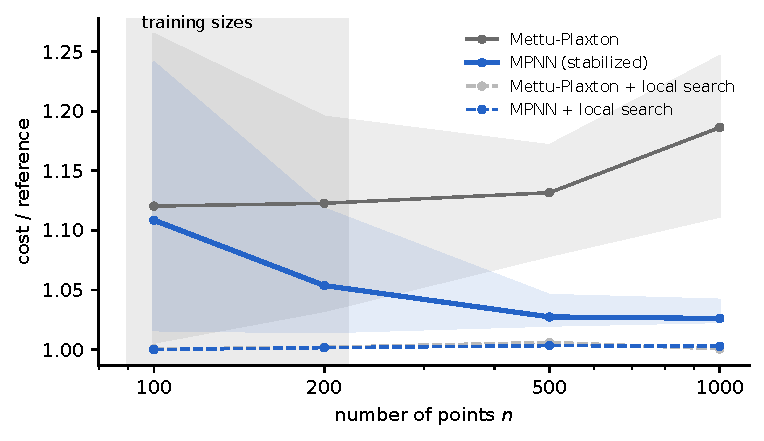
\includegraphics[width=0.85\linewidth]{../figuras/unifl.pdf}
\caption{Uniform facility location: cost of each method divided by a reference, as a function of
the number of points $n$ (log scale). The reference is the optimum proven by SCIP for $n\le 500$
(time limit 120--300~s) and the best solution found by any method for $n=1000$. A ratio of 1.00
is optimal; 1.10 is 10\% above. Lines are medians over the test instances (20, 20, 10 and 6 for
$n=100, 200, 500, 1000$); shaded bands are the 10th--90th percentiles, drawn only for the methods
without local search. \emph{Mettu--Plaxton}: the radius-based 3-approximation. \emph{MPNN
(stabilized)}: message-passing network trained without labels on an expected-cost loss, with
output probabilities clipped to $[0.01, 0.99]$ and gradient clipping (two seeds); the
pre-registered version collapsed in 3 of 4 seeds. Dashed lines add an add/drop/swap local search
to each. The grey band marks the sizes used for training. Source:
\texttt{results/pesquisa/unifl/}.}
\label{fig:unifl}
\end{figure}

\begin{figure}[h]\centering
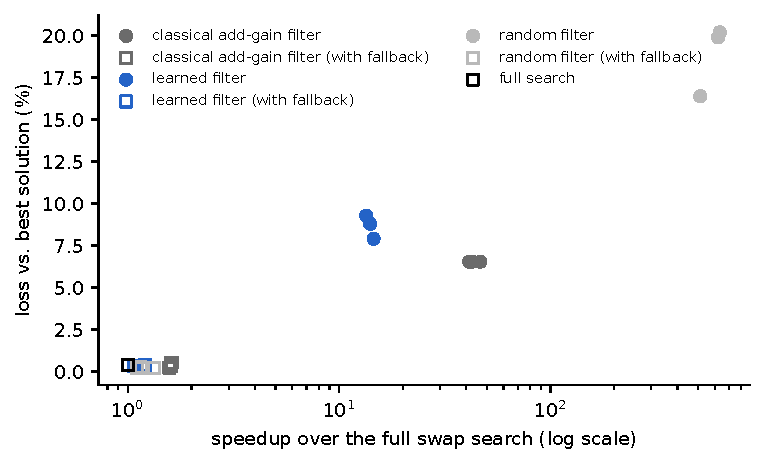
\includegraphics[width=0.85\linewidth]{../figuras/trocas.pdf}
\caption{Swap filters for the weighted $p$-median on synthetic road networks with $n=1000$ nodes
(5 networks, 3 random starts each). Each point is one filter configuration (8, 16 or 32 entering
candidates evaluated per iteration); coordinates are medians over the 15 runs. \emph{Horizontal
axis}: speedup, the running time of the full swap search divided by the running time of the
filtered search from the same start (log scale; 10 means ten times faster). \emph{Vertical axis}:
loss, the final cost relative to the best solution found by any configuration, in percent.
Filled circles stop when no filtered swap improves (the regime of the original papers); hollow
squares run one full sweep before stopping, which guarantees a true local optimum of the full
neighborhood. \emph{Classical add-gain filter}: ranks entering facilities by
$\sum_j w_j \max(0, d^{(1)}_j - d_{kj})$ and leaving facilities by their removal loss.
\emph{Learned filter}: two gradient-boosted regressors imitating the best exact swap gain, trained
on networks with $n=200$. Source: \texttt{results/pesquisa/swap\_v2/}.}
\label{fig:swaps}
\end{figure}

The common pattern is that the speedups reported for learned components often come from the
mechanism the learning plugs into (filtering candidate moves, decomposing the problem, embedding
a cheaper objective) rather than from the learning itself, which is why the classical
counterpart, given the same budget, is the necessary baseline.


\end{document}
